\documentclass{article}
\usepackage[utf8]{inputenc}

\title{KREPE Flight Computer Hardware Manual}
\author{Matt Ruffner}
\date{December 16, 2020}

\usepackage{url}
\usepackage{float}
\usepackage{natbib}
\usepackage{graphicx}
\usepackage{listings}
\usepackage{fullpage}
\usepackage{hyperref}
\hypersetup{
    colorlinks=true,
    linkcolor=blue,
    filecolor=magenta,      
    urlcolor=cyan,
}

\begin{document}

\maketitle
\tableofcontents
\listoffigures
\listoftables
\newpage


%%%%%%%%%%%%%%%%%%%%%%%%%%%%%%%%%%%%%%%%%%%%%%%%%%%%%%%%%%%%%%%%%%%%%%%%%%%%%%%%%%%%%%%%%
%%%%%%%%%%%%%%%%%%%%%%%%%%%%%%%%%%%%%%%%%%%%%%%%%%%%%%%%%%%%%%%%%%%%%%%%%%%%%%%%%%%%%%%%%
%%%%%%%%%%%%%%%%%%%%%%%%%%%%%%%%%%%%%%%%%%%%%%%%%%%%%%%%%%%%%%%%%%%%%%%%%%%%%%%%%%%%%%%%%
%%%%%%%%%%%%%%%%%%%%%%%%%%%%%%%%%%%%%%%%%%%%%%%%%%%%%%%%%%%%%%%%%%%%%%%%%%%%%%%%%%%%%%%%%
\section{Introduction}

This document contains information about the flight computer for the KREPE mission as well as the safety precautions taken to ensure the flight hardware is not a danger to the ISS or its astronauts. In addition to electrical designs and schematics, this document contains pin names, links to datasheets, and implementation notes. The following sections outline the subsystems of the flight computer, pin names for software usage, and datasheets. Other details about the power subsystem including battery type and rating are also included. 

The entire flight ready assembly is referred to as KREPE, which consists of a capsule containing the science (flight computer, batteries, etc.) and an metal shell known as KREM that acts as a Faraday cage inhibiting any inadvertent RF radiation from the probe. Both primary and secondary activation must occur for the capsule to become fully active and begin RF transmissions. To avoid accidental activation of hazardous subsystems, multiple secondary activation criteria must be met. Primary and secondary activation processes are discussed in sections ~\ref{sec:primary-activation},\ref{sec:secondary-activation}, and \ref{sec:radio-power-control}.

The subsystems of the flight computer are outlined in Sec.~\ref{sec:subsystems}. Pin definitions are listed with each hardware or sensor component along with any relevant information regarding safety or implementation. Electrical schematics, microcontroller reference cards, and a partslist are shown in  Appendices ~\ref{appa}, \ref{app:pinmap}, and \ref{app:partslist}, respectively.


\subsection{Primary Activation}
\label{sec:primary-activation}
Primary activation is triggered by a pin pulled out of KREPE by astronauts. Once the pin is pulled, a mechanical switch\footnote{\url{https://www.digikey.com/product-detail/en/omron-electronics-inc-emc-div/D2SW-3L1H/Z12268-ND/1811989}} is closed and the flight computer boots to dormant mode where it consumes minimal power. The Iridium radio is not powered on in dormant mode. After pulling the pull tab, a piece of copper tape is put over the hole and primary activation is the complete. Copper tape ensures the KREM is completely sealed with regard to EMI. 

A schematic showing battery protection and primary activation circuitry activation is shown in Fig. \ref{fig:activation-circuitry}. Less than 5 inches of copper 20 AWG PVC insulated wire is used to connect the batteries to the first power function (battery protection circuitry).


%The \texttt{POWER\_SW} header must closed for protected battery or USB voltage to be applied to the Teensy's VIN pin, powering on the system. The location of these connection points can be seen in Fig. \ref{fig:board-top} labelled on the silk screen in the left middle of the PCB. A rendering of the bottom of the board is shown in Fig. \ref{fig:board-bottom}.


\begin{figure}[H]
    \centering
    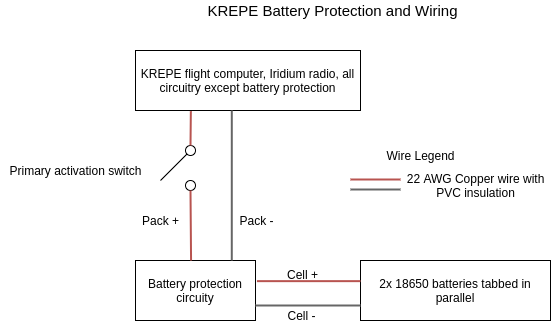
\includegraphics[width=0.8\textwidth]{images/krepe-electrical-overview.png}
    \caption{Activation and battery protection schematic overview.}
    \label{fig:activation-circuitry}
\end{figure}



%There is an low power 915MHz ISM band debug communication link that is only used during testing on the ground and is physically disconnected from power before once handed over for final integration. The \texttt{ISM\_SW} header is meant to enable and disable the RFM69 debug radio. The center 3.3V pin of this header is connected to the normally closed labeled pin, a GPIO pin is pulled high (see Fig. \ref{tab:pins_radio}). When the normally closed pin is connected to the center pin, the RFM69 is enabled. 




\subsection{Secondary Activation}
\label{sec:secondary-activation}
Once primary activation is complete and the flight computer is in dormant mode, a digital input to the flight computer is configured as an interrupt to sense when the KREM separates from around the capsule. When this interrupt is triggered, the flight computer checks the status of the thermocouples. If the thermocouples register a temperature that is sufficient to have melted the polycarbonate bolts that hold the KREM together, secondary activation occurs. If the temperature is not sufficient, the flight computer re-enters dormant mode. No radio transmissions are attempted before secondary activation. 

%Thermocouples and the KREM interrupt sensing subsystem are polled to check for conditions sufficient for secondary activation. As KREPE re-enters the atmosphere, heating of the metal KREM will melt the plastic bolts that hold it together. This ambient temperature increase of the probe is sensed by the thermal measurement subsystem and is one criteria for secondary activation. The presence of KREM around the probe is detected by capacitive sensors, this is the secondary criteria for secondary activation. Once the thermal and capacitive sensing subsystems have detected the separation of the metal enclosure, the Iridium radio is powered on and packet transmission begins.  

%An activation redundancy processor (ARP) was added in Rev. 1.1 of the flight computer, if the flight computer needs to be tested without the ARP, there is a solder jumper on the bottom of the PCB (SJ1) that, when shorted together, bypasses the AND gate that controls Iridium radio activation, reducing the system to single activation.




%%%%%%%%%%%%%%%%%%%%%%%%%%%%%%%%%%%%%%%%%%%%%%%%%%%%%%%%%%%%%%%%%%%%%%%%%%%%%%%%%%%%%%%%%
%%%%%%%%%%%%%%%%%%%%%%%%%%%%%%%%%%%%%%%%%%%%%%%%%%%%%%%%%%%%%%%%%%%%%%%%%%%%%%%%%%%%%%%%%
%%%%%%%%%%%%%%%%%%%%%%%%%%%%%%%%%%%%%%%%%%%%%%%%%%%%%%%%%%%%%%%%%%%%%%%%%%%%%%%%%%%%%%%%%
%%%%%%%%%%%%%%%%%%%%%%%%%%%%%%%%%%%%%%%%%%%%%%%%%%%%%%%%%%%%%%%%%%%%%%%%%%%%%%%%%%%%%%%%%
%%%%%%%%%%%%%%%%%%%%%%%%%%%%%%%%%%%%%%%%%%%%%%%%%%%%%%%%%%%%%%%%%%%%%%%%%%%%%%%%%%%%%%%%%
%%%%%%%%%%%%%%%%%%%%%%%%%%%%%%%%%%%%%%%%%%%%%%%%%%%%%%%%%%%%%%%%%%%%%%%%%%%%%%%%%%%%%%%%%
%%%%%%%%%%%%%%%%%%%%%%%%%%%%%%%%%%%%%%%%%%%%%%%%%%%%%%%%%%%%%%%%%%%%%%%%%%%%%%%%%%%%%%%%%
%%%%%%%%%%%%%%%%%%%%%%%%%%%%%%%%%%%%%%%%%%%%%%%%%%%%%%%%%%%%%%%%%%%%%%%%%%%%%%%%%%%%%%%%%
\section{Subsystems}
\label{sec:subsystems}

\iffalse
\subsection{Activation Redundancy Processor}
\label{actred}
Revision 1.1 of the KREPE flight computer adds a secondary safety processor as a schedule risk mitigation step should the KREM fail to provide the expected function as a Faraday cage and EMI testing shows unacceptable exceedances of EMI emissions. If the KREM functions as expected as a faraday cage, the safety processor hardware will be physically disabled and the ARP hardware will not be functional for flight. 

The SAMD21 Cortex-M0 safety processor polls the thermal monitoring subsystem to independently determine if temperature conditions for secondary activation are met. Figure~\ref{fig:actred} shows the interaction that the ARP has between the thermal monitoring hardware and the Iridium radio activation hardware, including the provisions for disabling it in the case that the KREM is an effective Faraday cage.

The rest of this subsection contains details related to board bring-up and programming.

%With the ARP in place, there are two separate CBCS in place in the KREPE capsule, meaning that an erroneous act from one CBCS is not sufficient to activate the iridium radio. 

\begin{figure}[H]
  \centering
  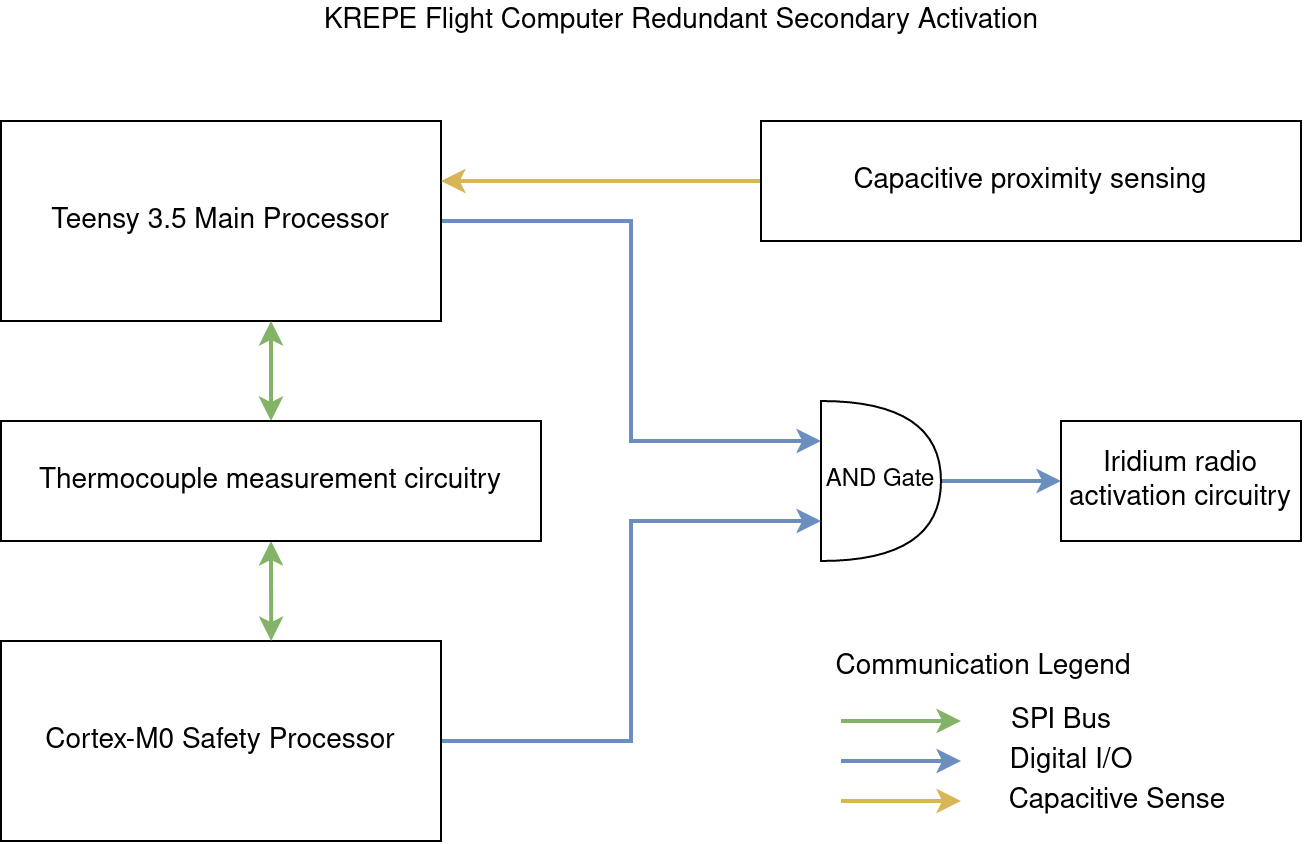
\includegraphics[width=0.7\textwidth]{images/redundant-activation.png}
  \caption{Secondary activation rendundancy provided by the safety processor.}
  \label{fig:actred}
\end{figure}

\paragraph{Bootloading the ARP}
The SAMD21 must be flashed with the UF2 bootloader \url{https://learn.adafruit.com/programming-microcontrollers-using-openocd-on-raspberry-pi}.

show picture of header for programming, reset pin, swclk, swdio pins. 
\paragraph{Programming the ARP}
The microUSB port next to the ARP (CN1) is used to upload program flash using the Arduino IDE. This is only possible once the bootloader has been flashed with OpenOCD.

\paragraph{Arduino Board File Modifications}
In order to have access to all GPIO used on the ARP, the Adafruit Trinket M0 default pin variant used by the Arduino IDE must be modified to include two more pins.
%\subsubsection{ARP Hardware Connections}
%Show which pins connect into the SPI bus and which goes to the AND gate for iridium activation.
%\begin{table}[H]
%	\centering
%	\begin{tabular}{l|l|l}
%		ARP Pin & Net Name     & Description \\
%		\hline 
%		1 & CS\_TC1      &   MAX31856 chip select, active low \texttt{OUTPUT}\\
%		13 & CS\_TC2      &   MAX31856 chip select, active low \texttt{OUTPUT}\\
%		0 & SEC\_CTRL\_2 &  Communication with Teensy \texttt{OUTPUT}\\
%		7 & SEC\_ACT     &  Activation signal \texttt{OUTPUT}\\
%		8 & SEC\_CTRL\_1 & Communication with Teensy  \texttt{INPUT} \\
%		23 & MUX0         &  TC MUX select \texttt{OUTPUT} \\
%		24 & MUX1         &  TC MUX select \texttt{OUTPUT} \\
%		21 & TC1\_FAULT   & MAX31856 fault signal  \texttt{INPUT} \\
%		22 & TC2\_FAULT   &   \texttt{OUTPUT} 
%	\end{tabular}
%	\caption{ARP pin assignment.}
%	\label{tab:arp-pins}
%\end{table}


%\subsection{Serial Interface Signals}
%\begin{table}[H]
%    \centering
%    \begin{tabular}{l|l|l}
%   Teensy Pin & Net Name &  Description \\
%    \hline \hline
%    
%        \hline
%    13 & SCLK     &  SPI Clock \\
%    12 & MISO     &  Master In Subject Out \\
%    11 & MOSI     &  Master Out Subject In \\
%    20 & CS@TC1 & MAX31856 chip select, active low \\
%    21 & CS@TC2 & MAX31856 chip select, active low  \\
%    9 & CS\_ISM     & RFM69 chip select, active low  \\
%    \hline
%    32 & TIRI     & Iridium TX UART \\
%    31 & RIRI      & Iridium RX UART \\
%    \hline
%    19 & SCL & I$^2$C bus clock \\
%    18 & SDA & I$^2$C bus data
%    \end{tabular}
%    \caption{Pins used with SPI, I$^2$C, and UART interfaces.}
%    \label{tab:pins_serial}
%\end{table}
\fi
\subsection{Radio Communications}

KREPE has two radios, a debug radio used for ground work and an Iridium satellite modem used both on the ground and during the mission. The following subsections explain the conditions necessary for enabling the satellite modem during the mission and also restate that the debug radio is physically disabled prior to final integration and is never powered on or used during the actual mission.

\subsubsection{Radio Power Control}
\label{sec:radio-power-control}
There are two inhibits to powering on the iridium, as denoted in Table~\ref{tab:radio-inhibits}. The separation of the KREM must be detected and the temperature of the capsule must be determined to be above the activation threshold temperature, $T_a$.
%Two indeAn AND gate controls the power to the solid state relay controlling power to the Iridium radio. The secondary processor is connected to the other input of this AND gate to make sure that erroneous action on behalf the Teensy (or secondary safety processor) is not able to solely activate the radio. In addition to the thermocouple measurements, another inhibit to powering on the Iridium radio is the detection of KREM separation, performed by capacitive sensing. Table \ref{tab:radio-inhibits} summarizes the inhibits to radio activation.


\begin{table}[H]
	\caption{Inhibits to Ididium radio activation.}
	\label{tab:radio-inhibits}
	\centering
	\begin{tabular}{l|l|l}
		Sensor & Monitored by     &  Description  \\
		\hline
		
		Thermocouples & Teensy  & Thermocouple temperature reported by Teensy\\
		%Thermocouples & ARP		& Thermocouple temperature reported by secondary ARP \\
		KREM Interrupt	 & Teensy  & KREM presence detected by Teensy
	\end{tabular}
	
\end{table}

%The following table shows the pin from the Teensy that activates the solid state relay controlling power to the Iridium radio.
%\begin{table}[H]
%	\centering
%	\caption{Teensy pin controlling power to the iridium satellite radio.}
%	\label{tab:pins-iridium}
%	\begin{tabular}{l|l|c|r}
%		Teensy Pin & Net Name     &  Description  & Teensy Configuration \\
%		\hline
%		23 & PRI\_ACT   & Primary Iridium activation, active high & \texttt{OUTPUT} 
%	\end{tabular}
%\end{table}


\subsubsection{Iriduim Radio}
We are using the A3LA-RS type modem seen on the NAL Research site~\footnote{ \url{http://www.nalresearch.com/IridiumHardware.html}}. The RF specifications, taken from the module's datasheet are shown in Fig. \ref{fig:iridium-rf-specs}.

\begin{figure}[H]
    \centering
    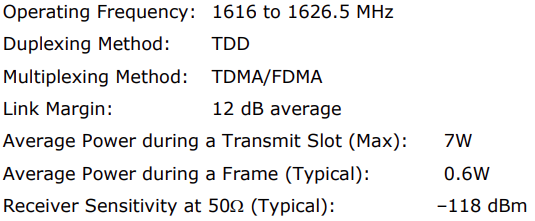
\includegraphics[width=0.5\textwidth]{images/iridium-rf-specs.png}
    \caption{RF specifications of the AL3A-RS Iridium modem.}
    \label{fig:iridium-rf-specs}
\end{figure}

\paragraph{Iridium Serial Interface}

A 3.3V TTL to RS232 adapter is needed to interface with the AL3A-RS. This small serial converter board is wired in between the flight computer and Iridium module. The serial converter uses a  MAX3232E RS-232 line driver and receiver~\footnote{\url{https://www.ti.com/product/MAX3232E}}.

\begin{figure}[H]
	\centering
	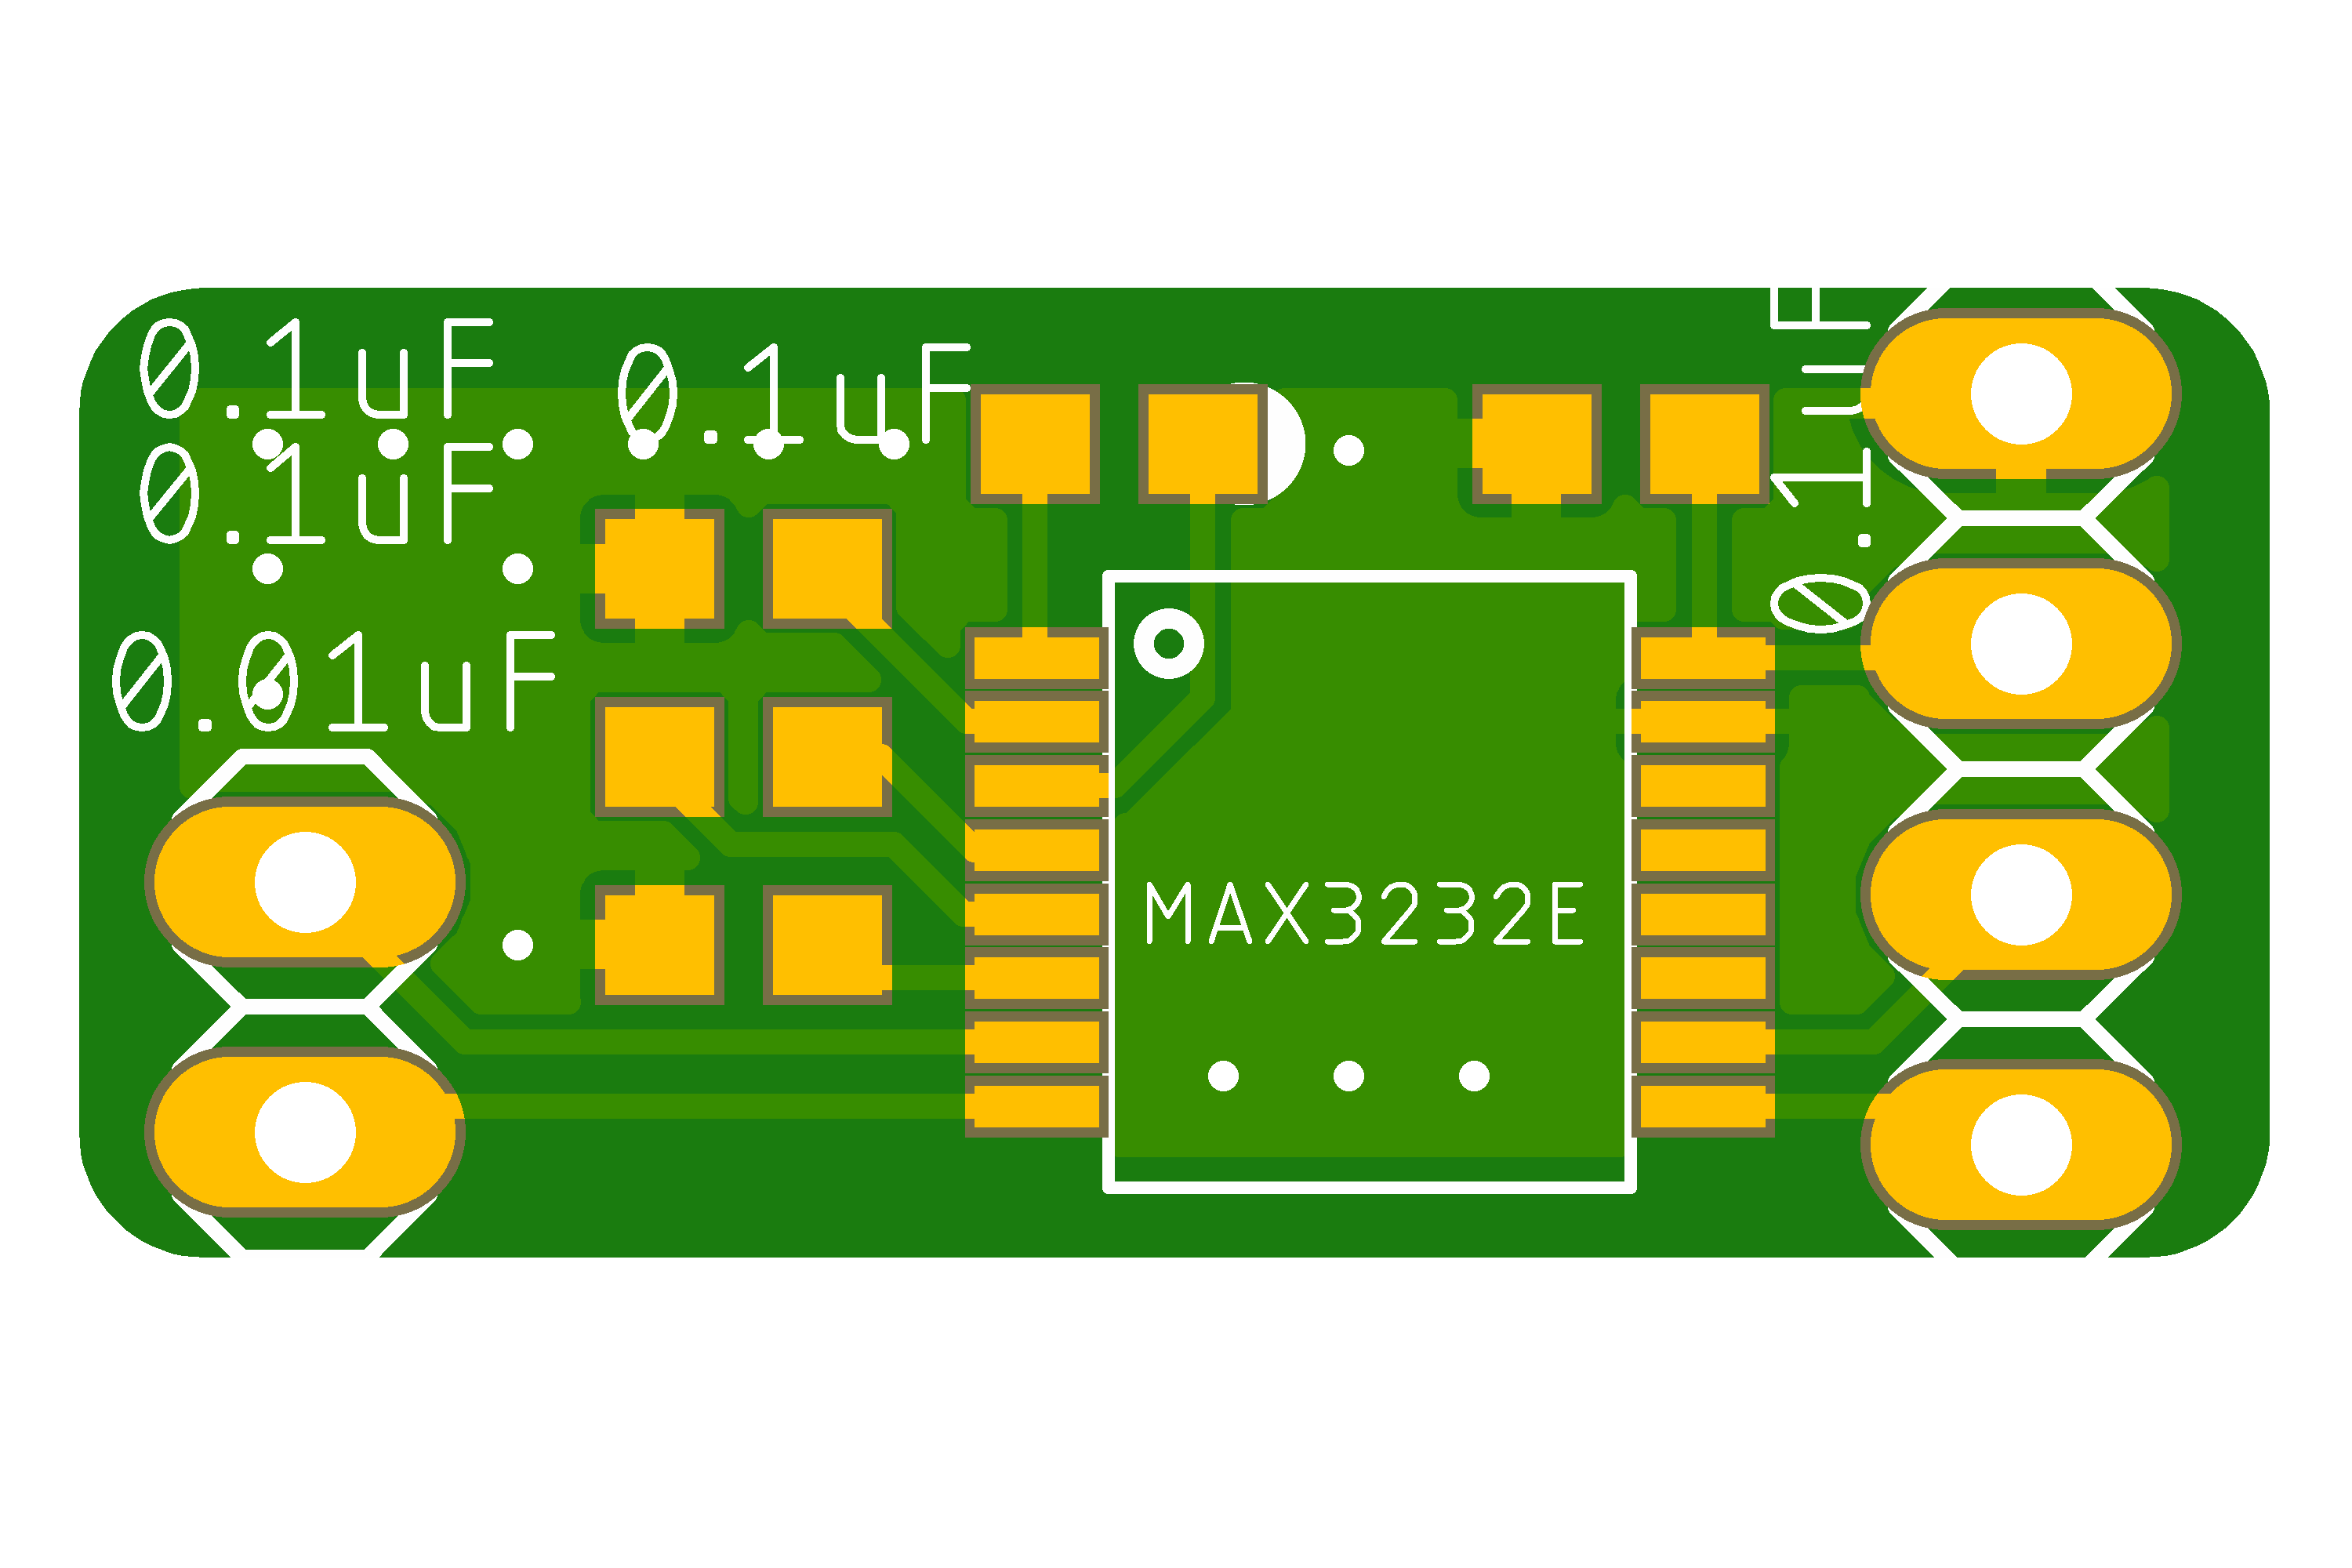
\includegraphics[width=0.3\textwidth]{images/serial-converter.png}
	\caption{TTL to RS232 serial converted module.}
	\label{fig:iridium-rf-specs}
\end{figure}



\subsubsection{Debug Radio}
The KREPE flight computer features a secondary debug radio used for ground testing that is not enabled for the real mission.  Maximum output power according to the radio datasheet \footnote{\url{https://cdn.sparkfun.com/datasheets/Wireless/General/RFM69HCW-V1.1.pdf}} is 100mW.
\begin{table}[H]
	\centering
	\caption{Radio module interface signals.}
	\label{tab:pins_radio}
	\begin{tabular}{l|l|l|l}
		Teensy Pin & Net Name  & Description   & Teensy Configuration \\
		\hline 
		28 & RESET\_ISM  &  Pull low to enable RFM69   & \texttt{OUTPUT} \\
		29 & INT\_ISM    &  GPIO0 interrupt from RFM69 & \texttt{INPUT} \\
		33 & RADIO\_OFF\_SIG & Pulled high when the RFM69 is disabled & \texttt{INPUT} \\
	\end{tabular}
\end{table}
The datasheet for this antenna can be found at  \url{https://cdn.taoglas.com/datasheets/FXP290.07.0100A.pdf}. 
  


\subsection{Thermal Measurement}
The thermal measurement subsystem is used to take readings from up to eight thermocouples (TCs) to characterize the temperature profile that is experienced by the probe upon re-entry. As KREPE heats during re-entry, this subsystem detect the increase in temperature and is also used as a secondary activation criteria. Table~\ref{tab:pins_thermo} shows the pins used to control the TC conversion chips and analog multiplexers making multi-TC readings possible.

\begin{table}[H]
    \centering
    \caption{Analog mux selection and thermocouple fault status pins.}
    \label{tab:pins_thermo}
    \begin{tabular}{c|c|c|r}
    Teensy Pin & Net Name  & Description   & Teensy Configuration \\
    \hline 
    16 & MUX0 & MUX select pin 0 & \texttt{OUTPUT} \\
    17 & MUX1 & MUX select pin 1 & \texttt{OUTPUT} \\
    25 & TC1\_FAULT & U13 fault (active low) & \texttt{INPUT} \\
    26 & TC2\_FAULT & U12 fault (active low) & \texttt{INPUT} \\ 
    \end{tabular}
\end{table}

\subsubsection{Thermocouple Connections}
The 8 TC connections are done with 2 analog multiplexers IC1 and IC3 (MUX1 and MUX2). The MUX select pins go to both of these chips to select a certain channel. The table of MUX(0/1) select values versus two selected TCs are shown in Table \ref{tab:tc-mux-sel}.

\begin{table}[H]
  \centering
  \caption{Truth table for multiplexer select pins and their relation to the pairs of TC that are selected.}
  \label{tab:tc-mux-sel}
  \begin{tabular}{c | c | c}
    MUX0 & MUX1 & TC number \\
    \hline
    0 & 0 & 1, 5 \\
    0 & 1 & 2, 6 \\
    1 & 0 & 3, 7 \\
    1 & 1 & 4, 8
  \end{tabular}
\end{table}
%
Pin connections on headers P1 and P2 show the connections for TC 1-8 lead wire pairs. Figure \ref{fig:tc-conn} shows the pinout on the silkscreen.
%
\begin{figure}[H]
    \centering
    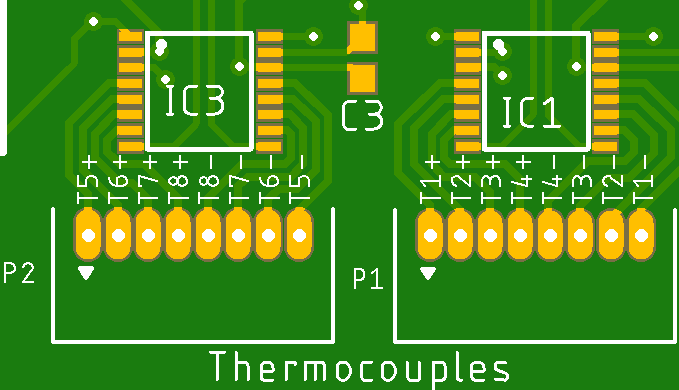
\includegraphics[width=0.5\textwidth]{images/krepe-thermocouples.png}
    \caption{Thermocouple connection wiring with resepect to the analog mux chips IC3 (MUX2) and IC1 (MUX1).}
    \label{fig:tc-conn}
\end{figure}


%%%%%%%%%%%%%%%%%%%%%%%%%%%%%%%%%%%%%%%%%%%%%%%%%%%%%%%%%%%%%
\subsection{Visual Status Indicators}
The KREPE flight computer features several light emitting diodes (LEDs) to provide visual feedback during ground testing. Pin mappings and intended information denoted by each LED is shown in Table \ref{tab:pins_leds}.
\begin{table}[H]
	\centering
	\caption{Debug LED Connections.}
	\label{tab:pins_leds}
	\begin{tabular}{l|l|l}
		Teensy Pin & Net Name     & Teensy Configuration \\
		\hline 
		3 & LED1 - IRIDIUM ON        &   \texttt{OUTPUT}\\
		4 & LED2 - IRIDIUM SIGNAL OK       &   \texttt{OUTPUT}\\
		5 & LED3 - IRIDIUM RADIO TRANSMITTING       &   \texttt{OUTPUT}\\
		6 & LED4 - ISM RADIO TRANSMITTING       &   \texttt{OUTPUT}\\
		7 & LED5 - GENERAL ACTIVITY       &   \texttt{OUTPUT}
	\end{tabular}
\end{table}


%%%%%%%%%%%%%%%%%%%%%%%%%%%%%%%%%%%%%%%%%%%%%%%%%%%%%%%%%%%%%
\subsection{Auxillary Sensors}
The KREPE flight computer features several auxillary sensors that will be used to better characterize reentry. Measurements from an ADXL377 3-axis $\pm$200g accelerometer, ICM-20948 9-axis IMU, and DSP310 barometric pressure sensor are collected after secondary activation. Measurements from these auxiliary sensors are not used for activation.

\begin{table}[H]
    \centering
    \caption{Pins connecting to the ADXL377 and ICM-20948.}
    \label{tab:pins_motionsensor}
    \begin{tabular}{c|c|c|r}
    Teensy Pin & Net Name  & Description   & Teensy Configuration \\
    \hline 
    36 A17 & XOUT & Analog out from accel (x axis) & \texttt{INPUT} \\
    37 A18 & YOUT & Analog out from accel (y axis) & \texttt{INPUT} \\
    38 A19 & ZOUT & Analog out from accel (z axis) & \texttt{INPUT} \\
    35 & INT & Interrupt from ICM-20948 & \texttt{INPUT} \\
    34 & FSYNC & Synchronization signal to ICM-20948 & \texttt{OUTPUT} 
    \end{tabular}
\end{table}

%\paragraph{Barometric Pressure Sensor}
%Version 1.1 of the flight computer features an Infineon DSP310 barometric pressure and temperature sensor connected to the SPI bus with active low chip select on pin 8 of the Teensy. This sensor is not used for activation detection. 



%%%%%%%%%%%%%%%%%%%%%%%%%%%%%%%%%%%%%%%%%%%%%%%%%%%%%%%%%%%%%%%55
\subsection{Power and Batteries}
Batteries are provided by JSC and rated at 3200mAh. System power is provided by two of these cells tabbed in parallel (tabbing performed and documented by JSC). Battery classification, product, and model number can be seen in Fig. \ref{fig:bat-spec} (taken from battery specification sheet).

\begin{figure}[h!]
	\centering
	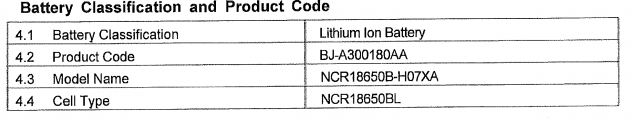
\includegraphics[width=12cm]{images/battery-spec.png}
	\label{fig:bat-spec}
	\caption{Sanyo battery specifications from the datasheet.}
\end{figure}

Charge current is limited to to 450 milliamps (mA), a charge rate of $C/12$ with the two (2) 3200 milliamp-hour (mAh) system  Battery Charge power can be delivered via Teensy USB or the \texttt{CHARGE} header. Charging input voltage is expected to be 5 volts. Charge voltage to the batteries is regulated to 4.2 volts by the charge management IC, an MCP73831\footnote{ (\url{https://www.microchip.com/wwwproducts/en/MCP73831})}, with status connections to the Teensy as shown in Table \ref{tab:pins-battery}. 

charging when not installed vs charging when installed.

Charging is only performed on the ground and there is no provision for charging in flight. Schematics and electrical connections are shown in Fig. \ref{fig:page1-3} in Appendix \ref{appa}.

\subsubsection{Battery Status Interface}
\begin{table}[H]
    \centering
    \caption{Pins to monitor battery voltage and charging status.}
	\label{tab:pins-battery}
    \begin{tabular}{c|c|c|r}
    Teensy Pin & Net Name  & Description   & Teensy Configuration \\
    \hline 
    14 & BAT\_STAT & LiPo charge state & \texttt{OUTPUT} \\
    22 A8 & BAT\_SENSE    &  Halved battery voltage for monitoring &   \texttt{INPUT} 
    \end{tabular}
\end{table}

\subsubsection{Battery Protection}
Protection circuitry is implemented on the flight board to support 2P1S LiIon packs for system power. We are using a DW108 Voltage and Current Protection IC \footnote{\url{https://cdn.sparkfun.com/assets/learn_tutorials/2/5/1/DW01-P_DataSheet_V10.pdf}}.


\begin{figure}[H]
	\centering
	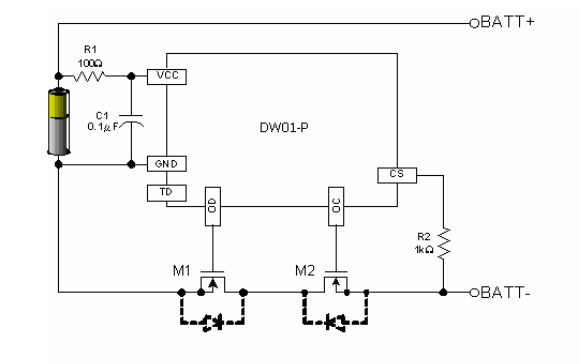
\includegraphics[width=0.6\textwidth]{images/dw108.png}
	\caption{Battery protection circuitry.}
	\label{fig:bat-protec}
\end{figure}



Protection circuitry as implemented on the KREPE flight computer PCB is shown in Fig. \ref{fig:bat-protec}. Our two batteries are in parallel where the battery image is shown in Fig. \ref{fig:bat-protec}, and BATT+ and BATT- face system power i.e. to the flight computer. This protection circuitry is upstream of the primary activation switch. The battery protection PCB can be seen in Fig. \ref{fig:bat-protect}.


\begin{figure}[H]
	\centering
	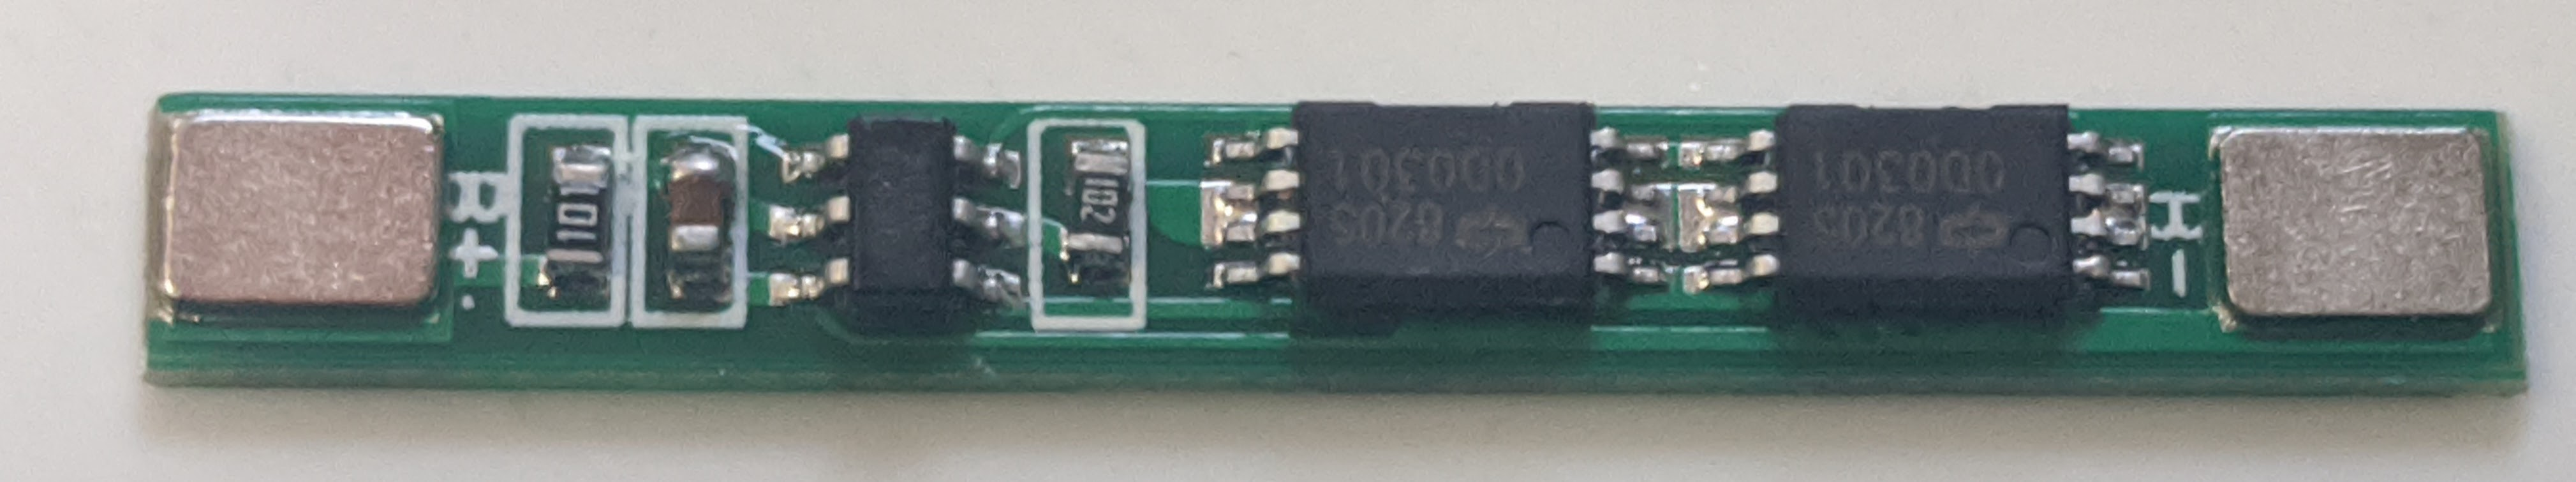
\includegraphics[width=0.5\textwidth]{images/new_batt_prot.png}
	\caption{Battery protection PCB.}
	\label{fig:bat-protect}
\end{figure}


\paragraph{Over-current protection}
The battery protection PCB can be seen preventing over current draw in Fig. \ref{fig:over-current}. After 6 milliseconds, the battery cells are disconnected from the output and current draw 


\begin{figure}[H]
	\centering
	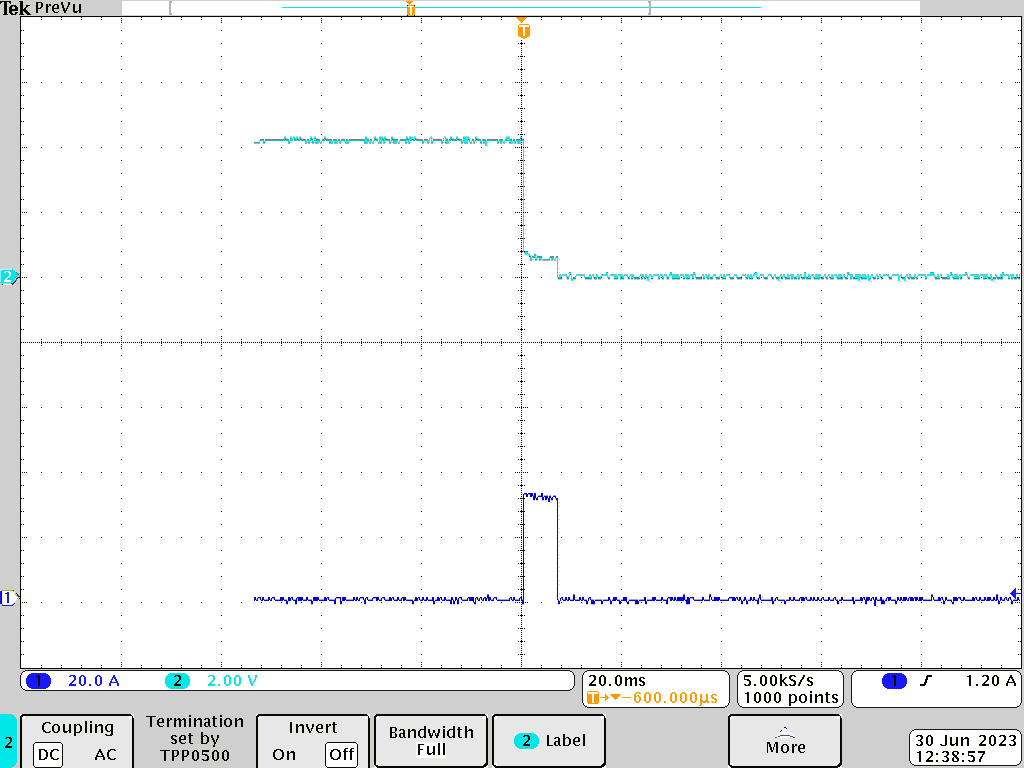
\includegraphics[width=0.9\textwidth]{images/over-current.png}
	\caption{The battery protection circuity disconnecting the cells after 6ms of over current condition. Blue: current. Purple: pack voltage.}
	\label{fig:over-current}
\end{figure}




%%%%%%%%%%%%%%%%%%%%%%%%%%%%%%%%%%%%%%%%%%%%%%%%%%%%%%%%%%%%%%%%%%%%%%%%%%%%%%%%%%%
%%%%%%%%%%%%%%%%%%%%%%%%%%%%%%%%%%%%%%%%%%%%%%%%%%%%%%%%%%%%%%%%%%%%%%%%%%%%%%%%%%%
%%%%%%%%%%%%%%%%%%%%%%%%%%%%%%%%  APPENDIX
%%%%%%%%%%%%%%%%%%%%%%%%%%%%%%%%%%%%%%%%%%%%%%%%%%%%%%%%%%%%%%%%%%%%%%%%%%%%%%%%%%%
%%%%%%%%%%%%%%%%%%%%%%%%%%%%%%%%%%%%%%%%%%%%%%%%%%%%%%%%%%%%%%%%%%%%%%%%%%%%%%%%%%%
\appendix


\section{Schematics}
\label{appa}

\begin{figure}[H]
    \centering
    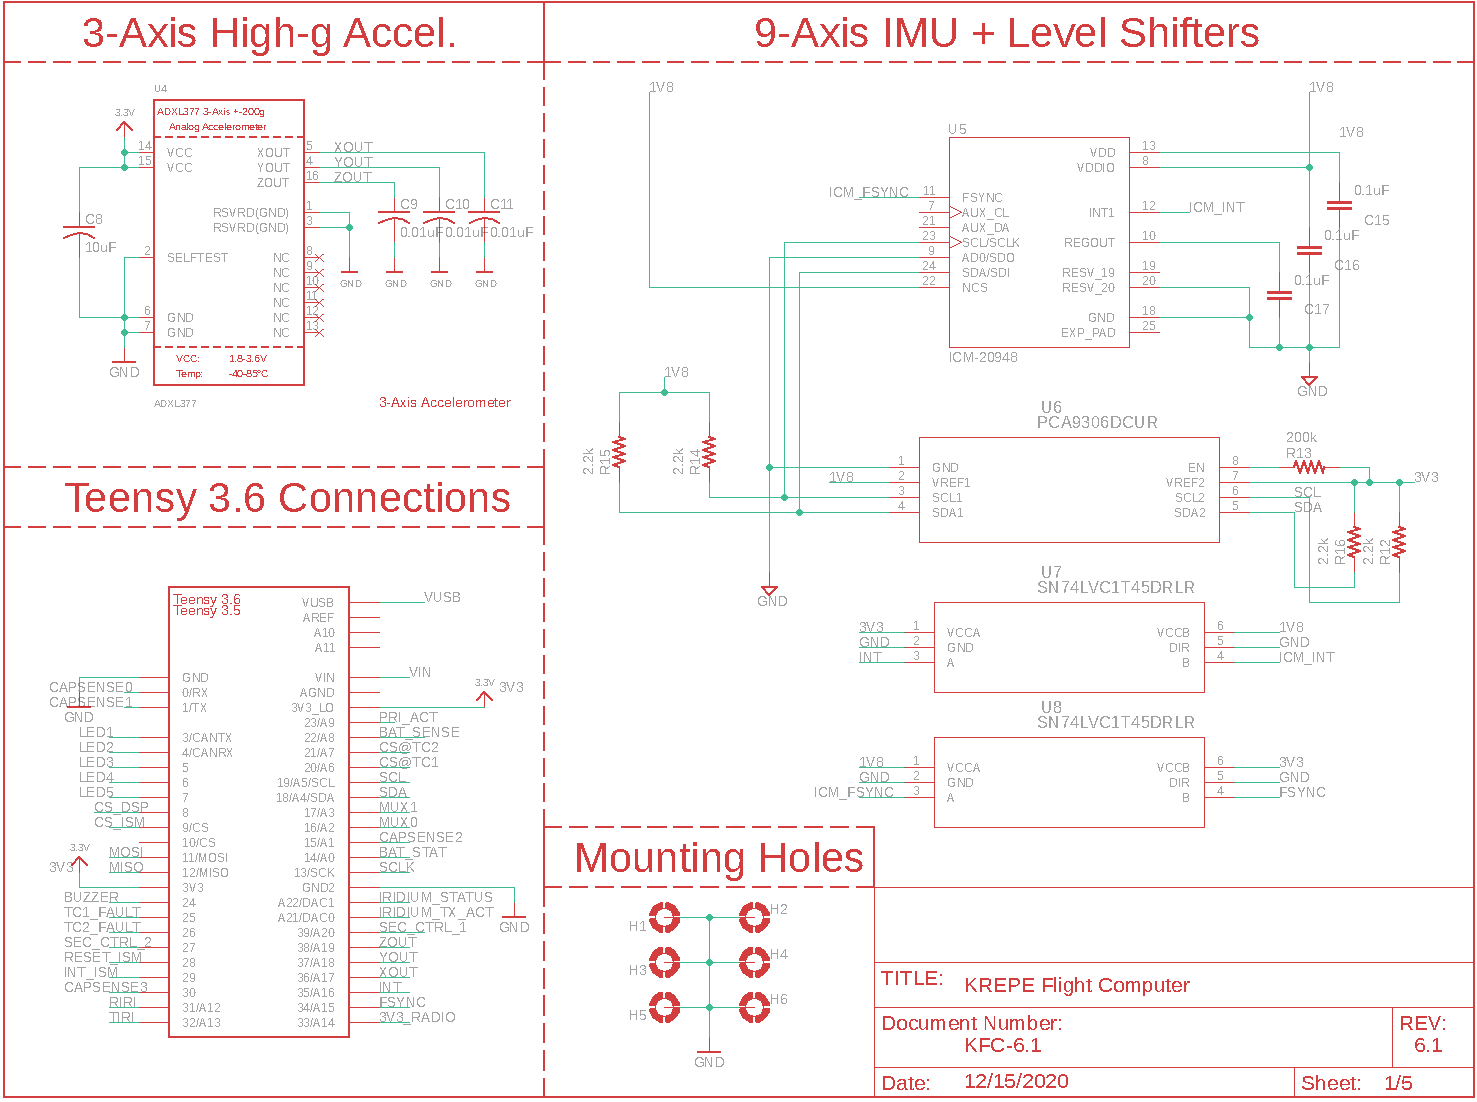
\includegraphics[width=\textwidth]{images/page1.png}
    \caption{Page one of schematics.}
    \label{fig:page1-2}
\end{figure}

\begin{figure}[H]
    \centering
    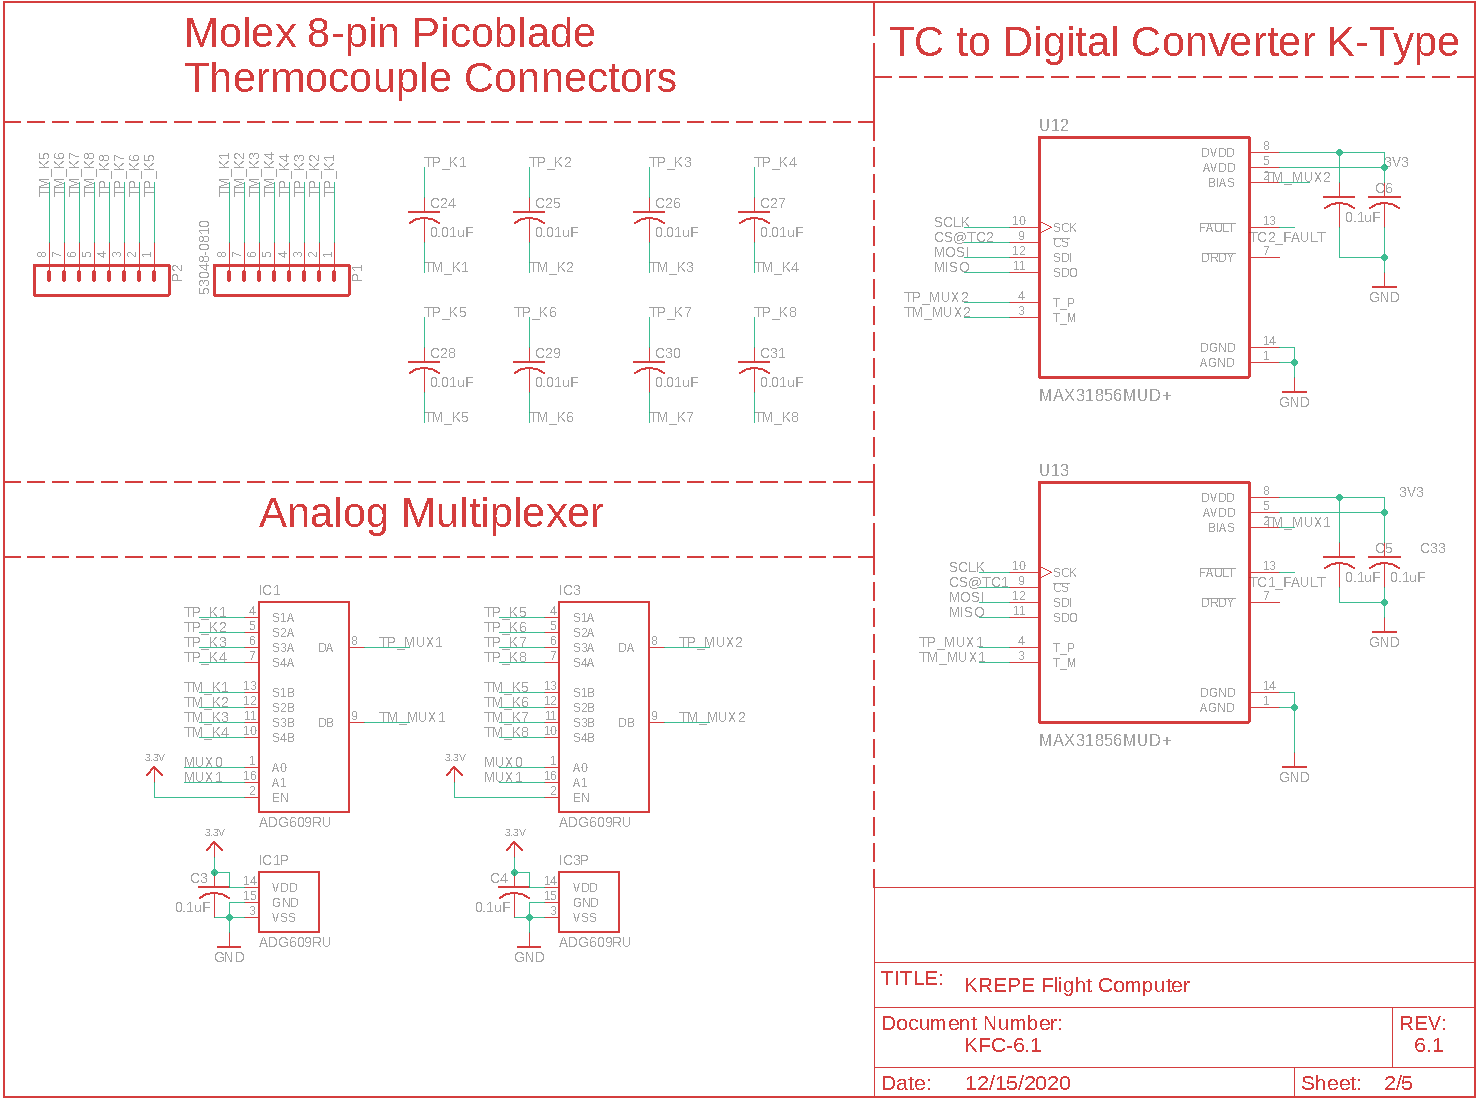
\includegraphics[width=\textwidth]{images/page2.png}
    \caption{Page two of schematics.}
    \label{fig:page1_1}
\end{figure}

\begin{figure}[H]
    \centering
    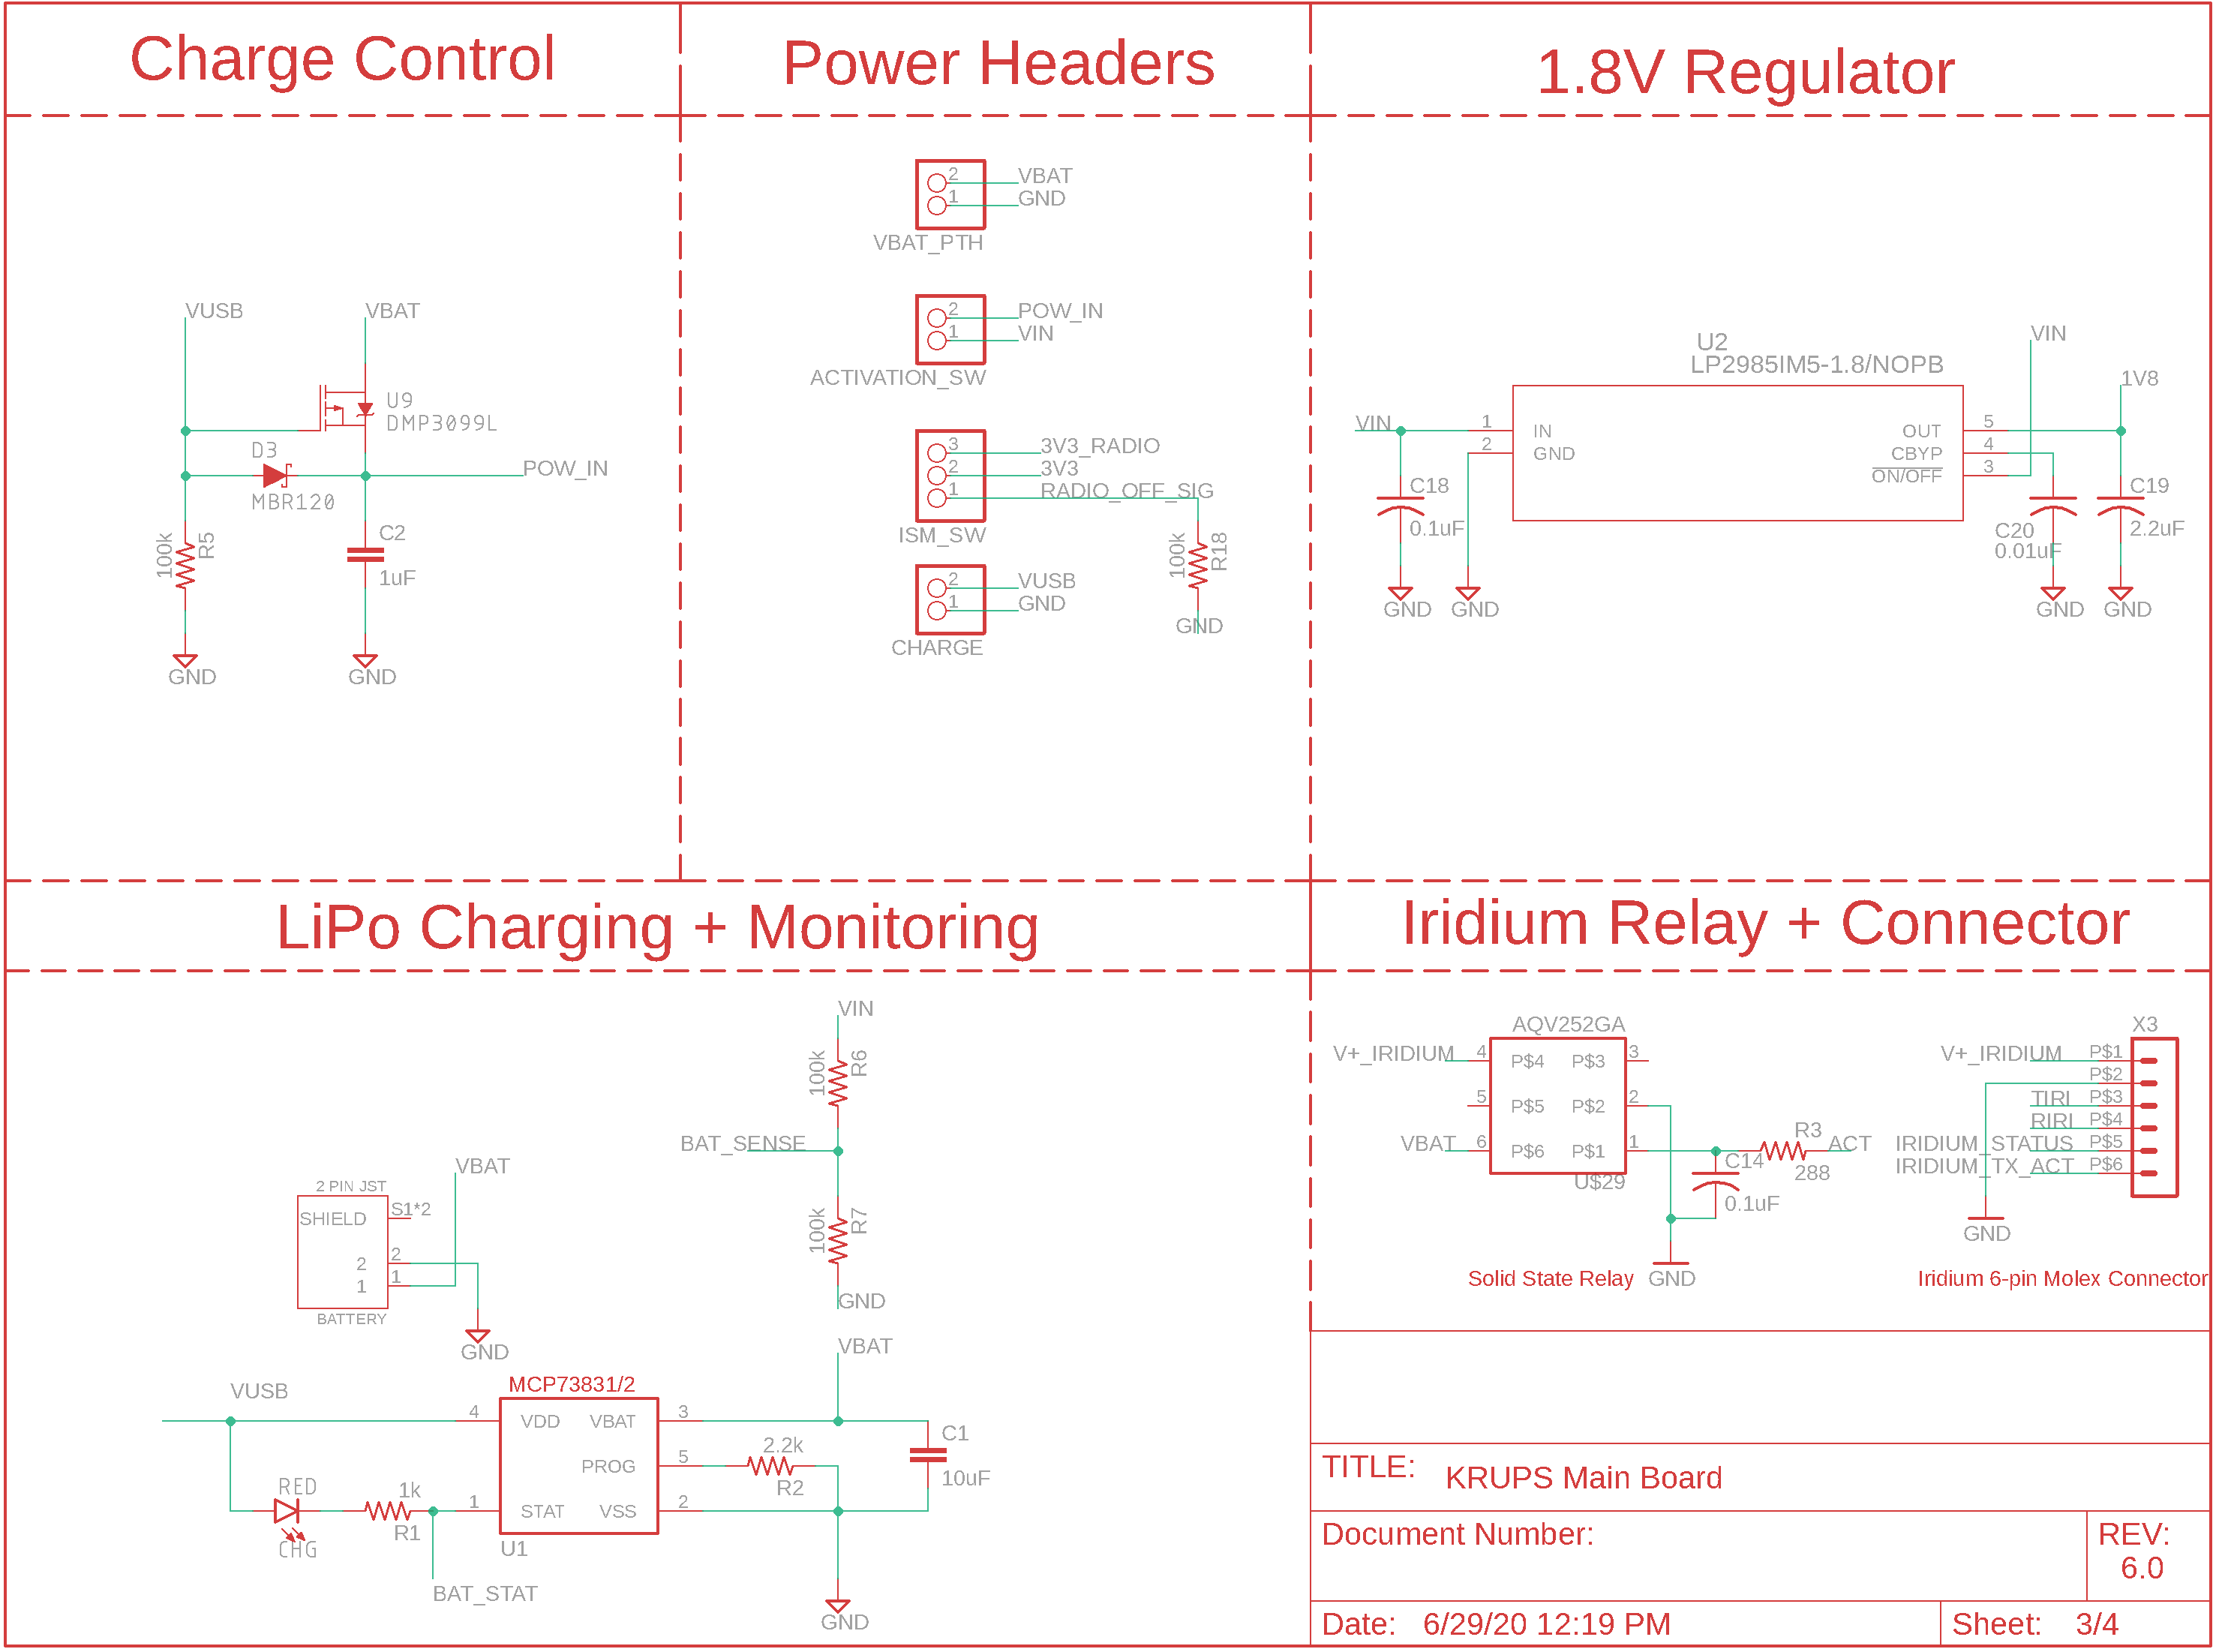
\includegraphics[width=\textwidth]{images/page3.png}
    \caption{Page three of schematics.}
    \label{fig:page1-3}
\end{figure}

\begin{figure}[H]
    \centering
    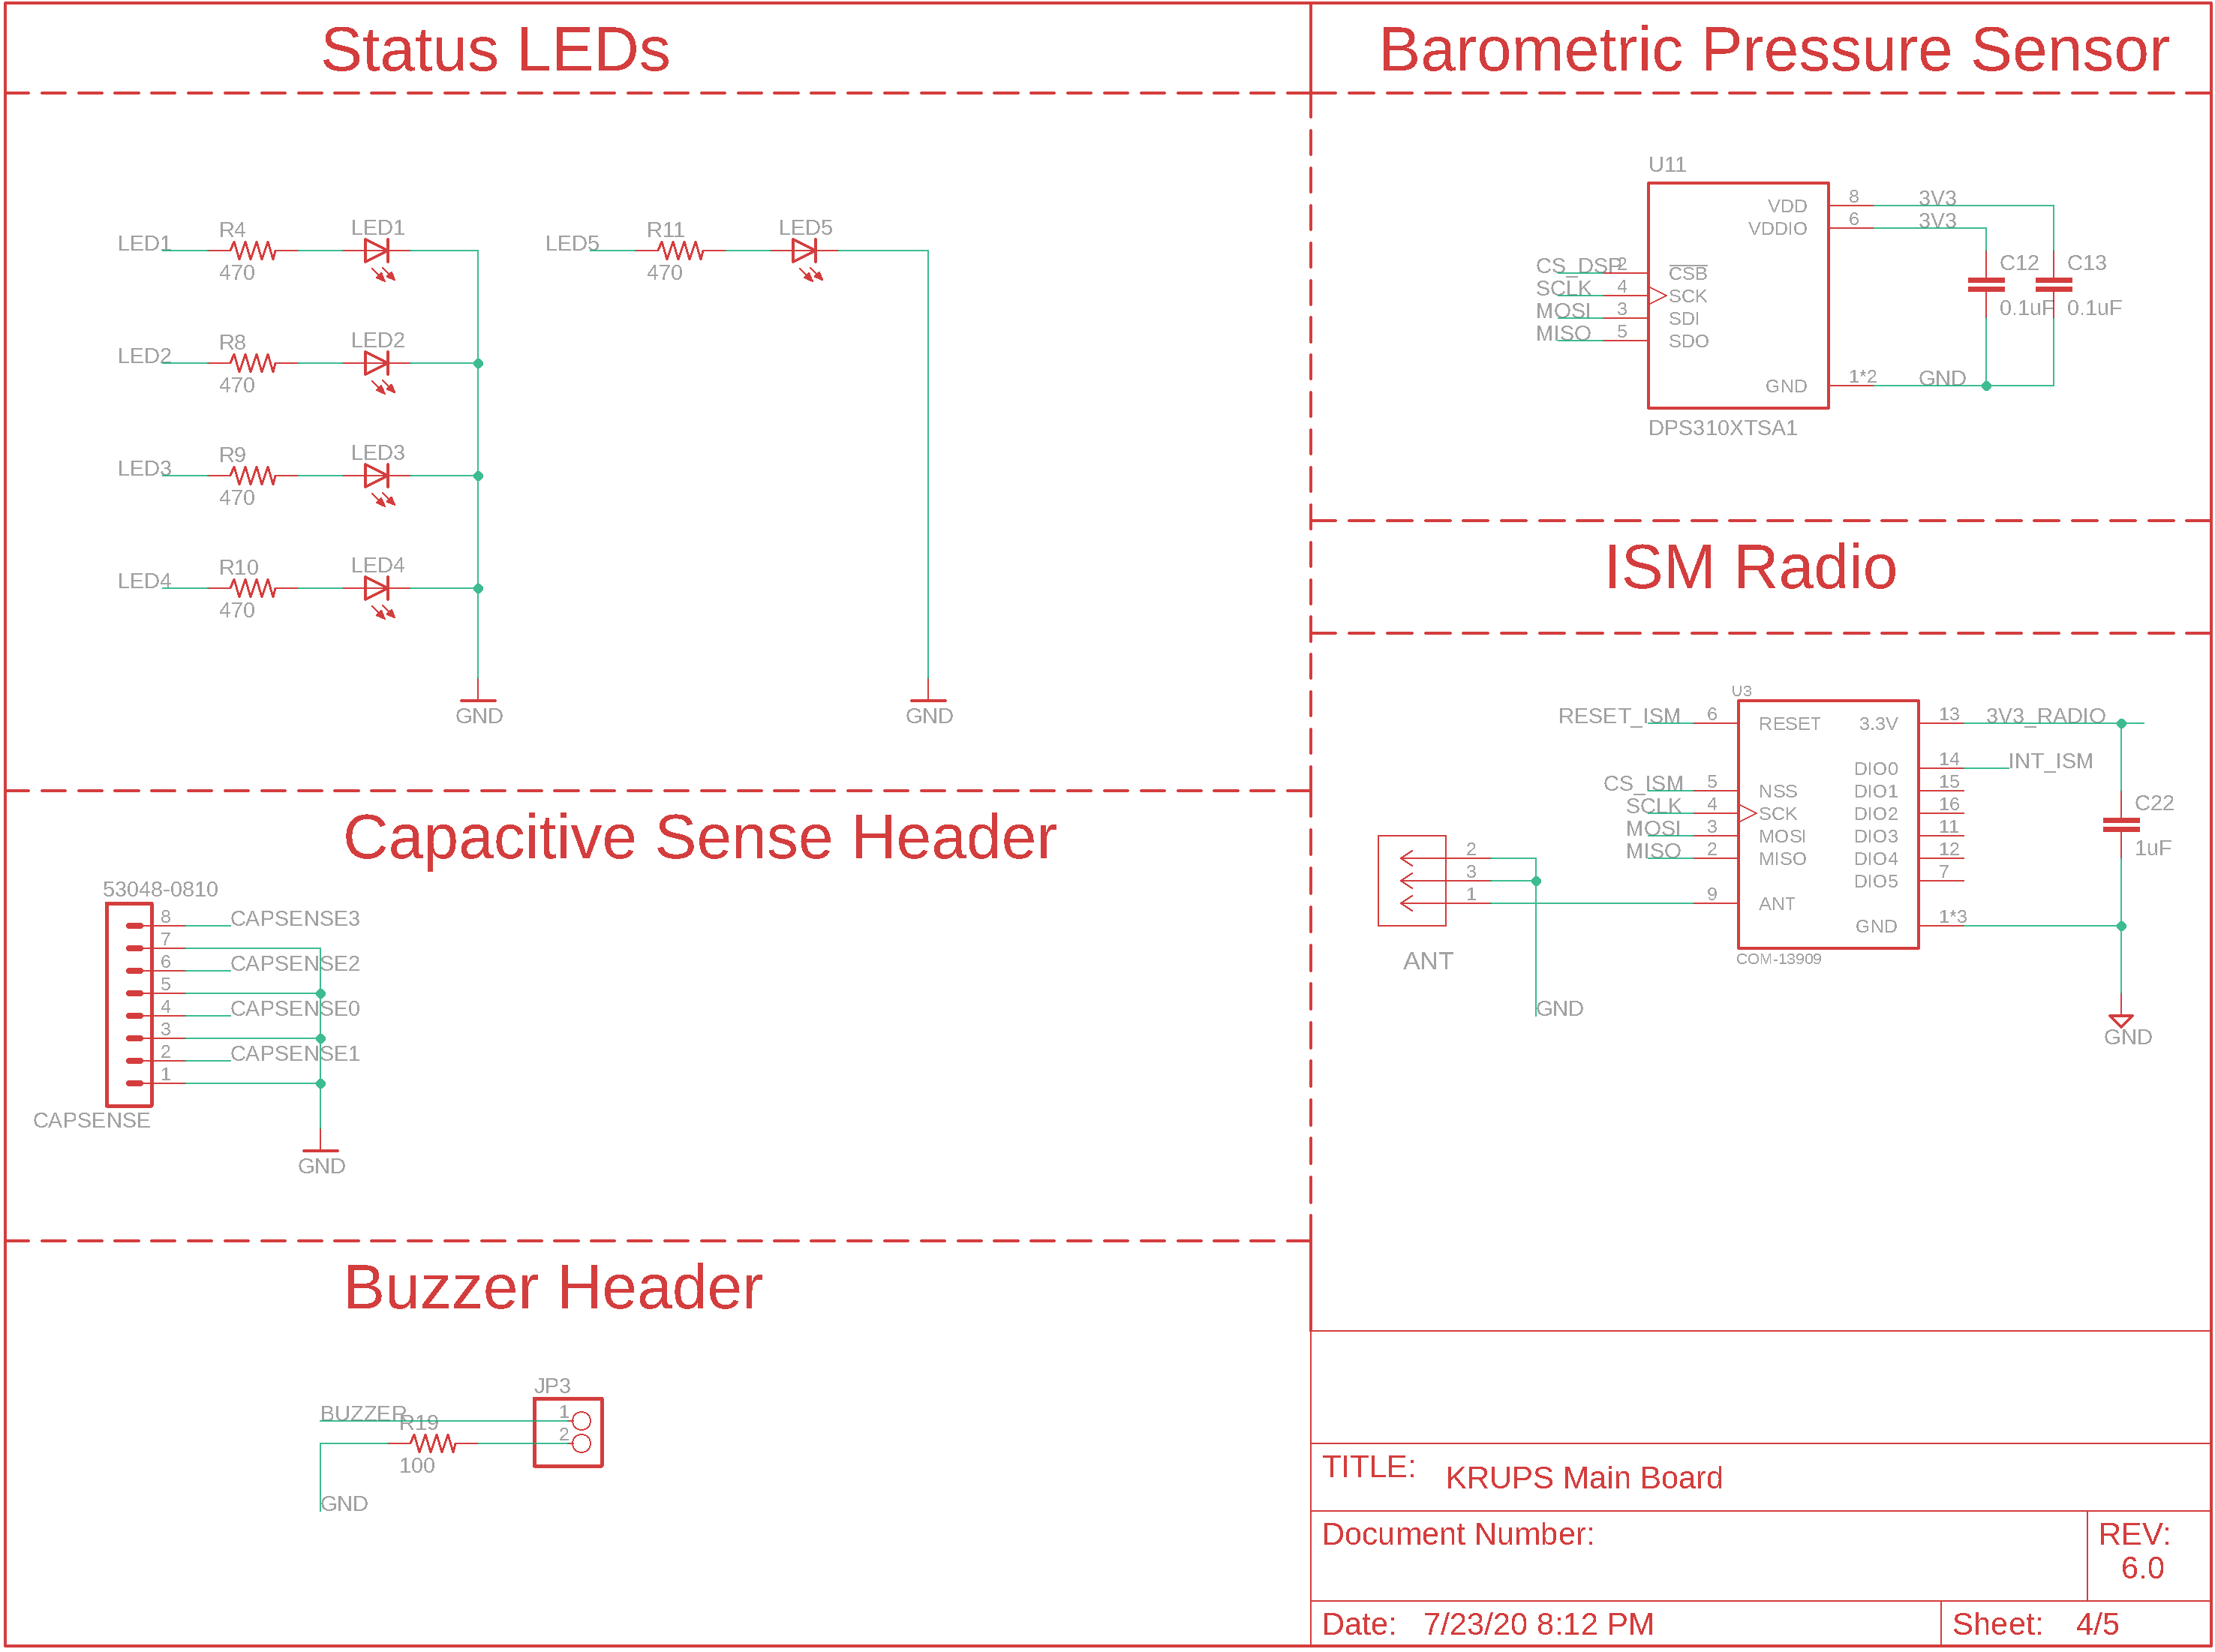
\includegraphics[width=\textwidth]{images/page4.png}
    \caption{Page four of schematics.}
    \label{fig:page1-4}
\end{figure}


%\begin{figure}[H]
%    \centering
%    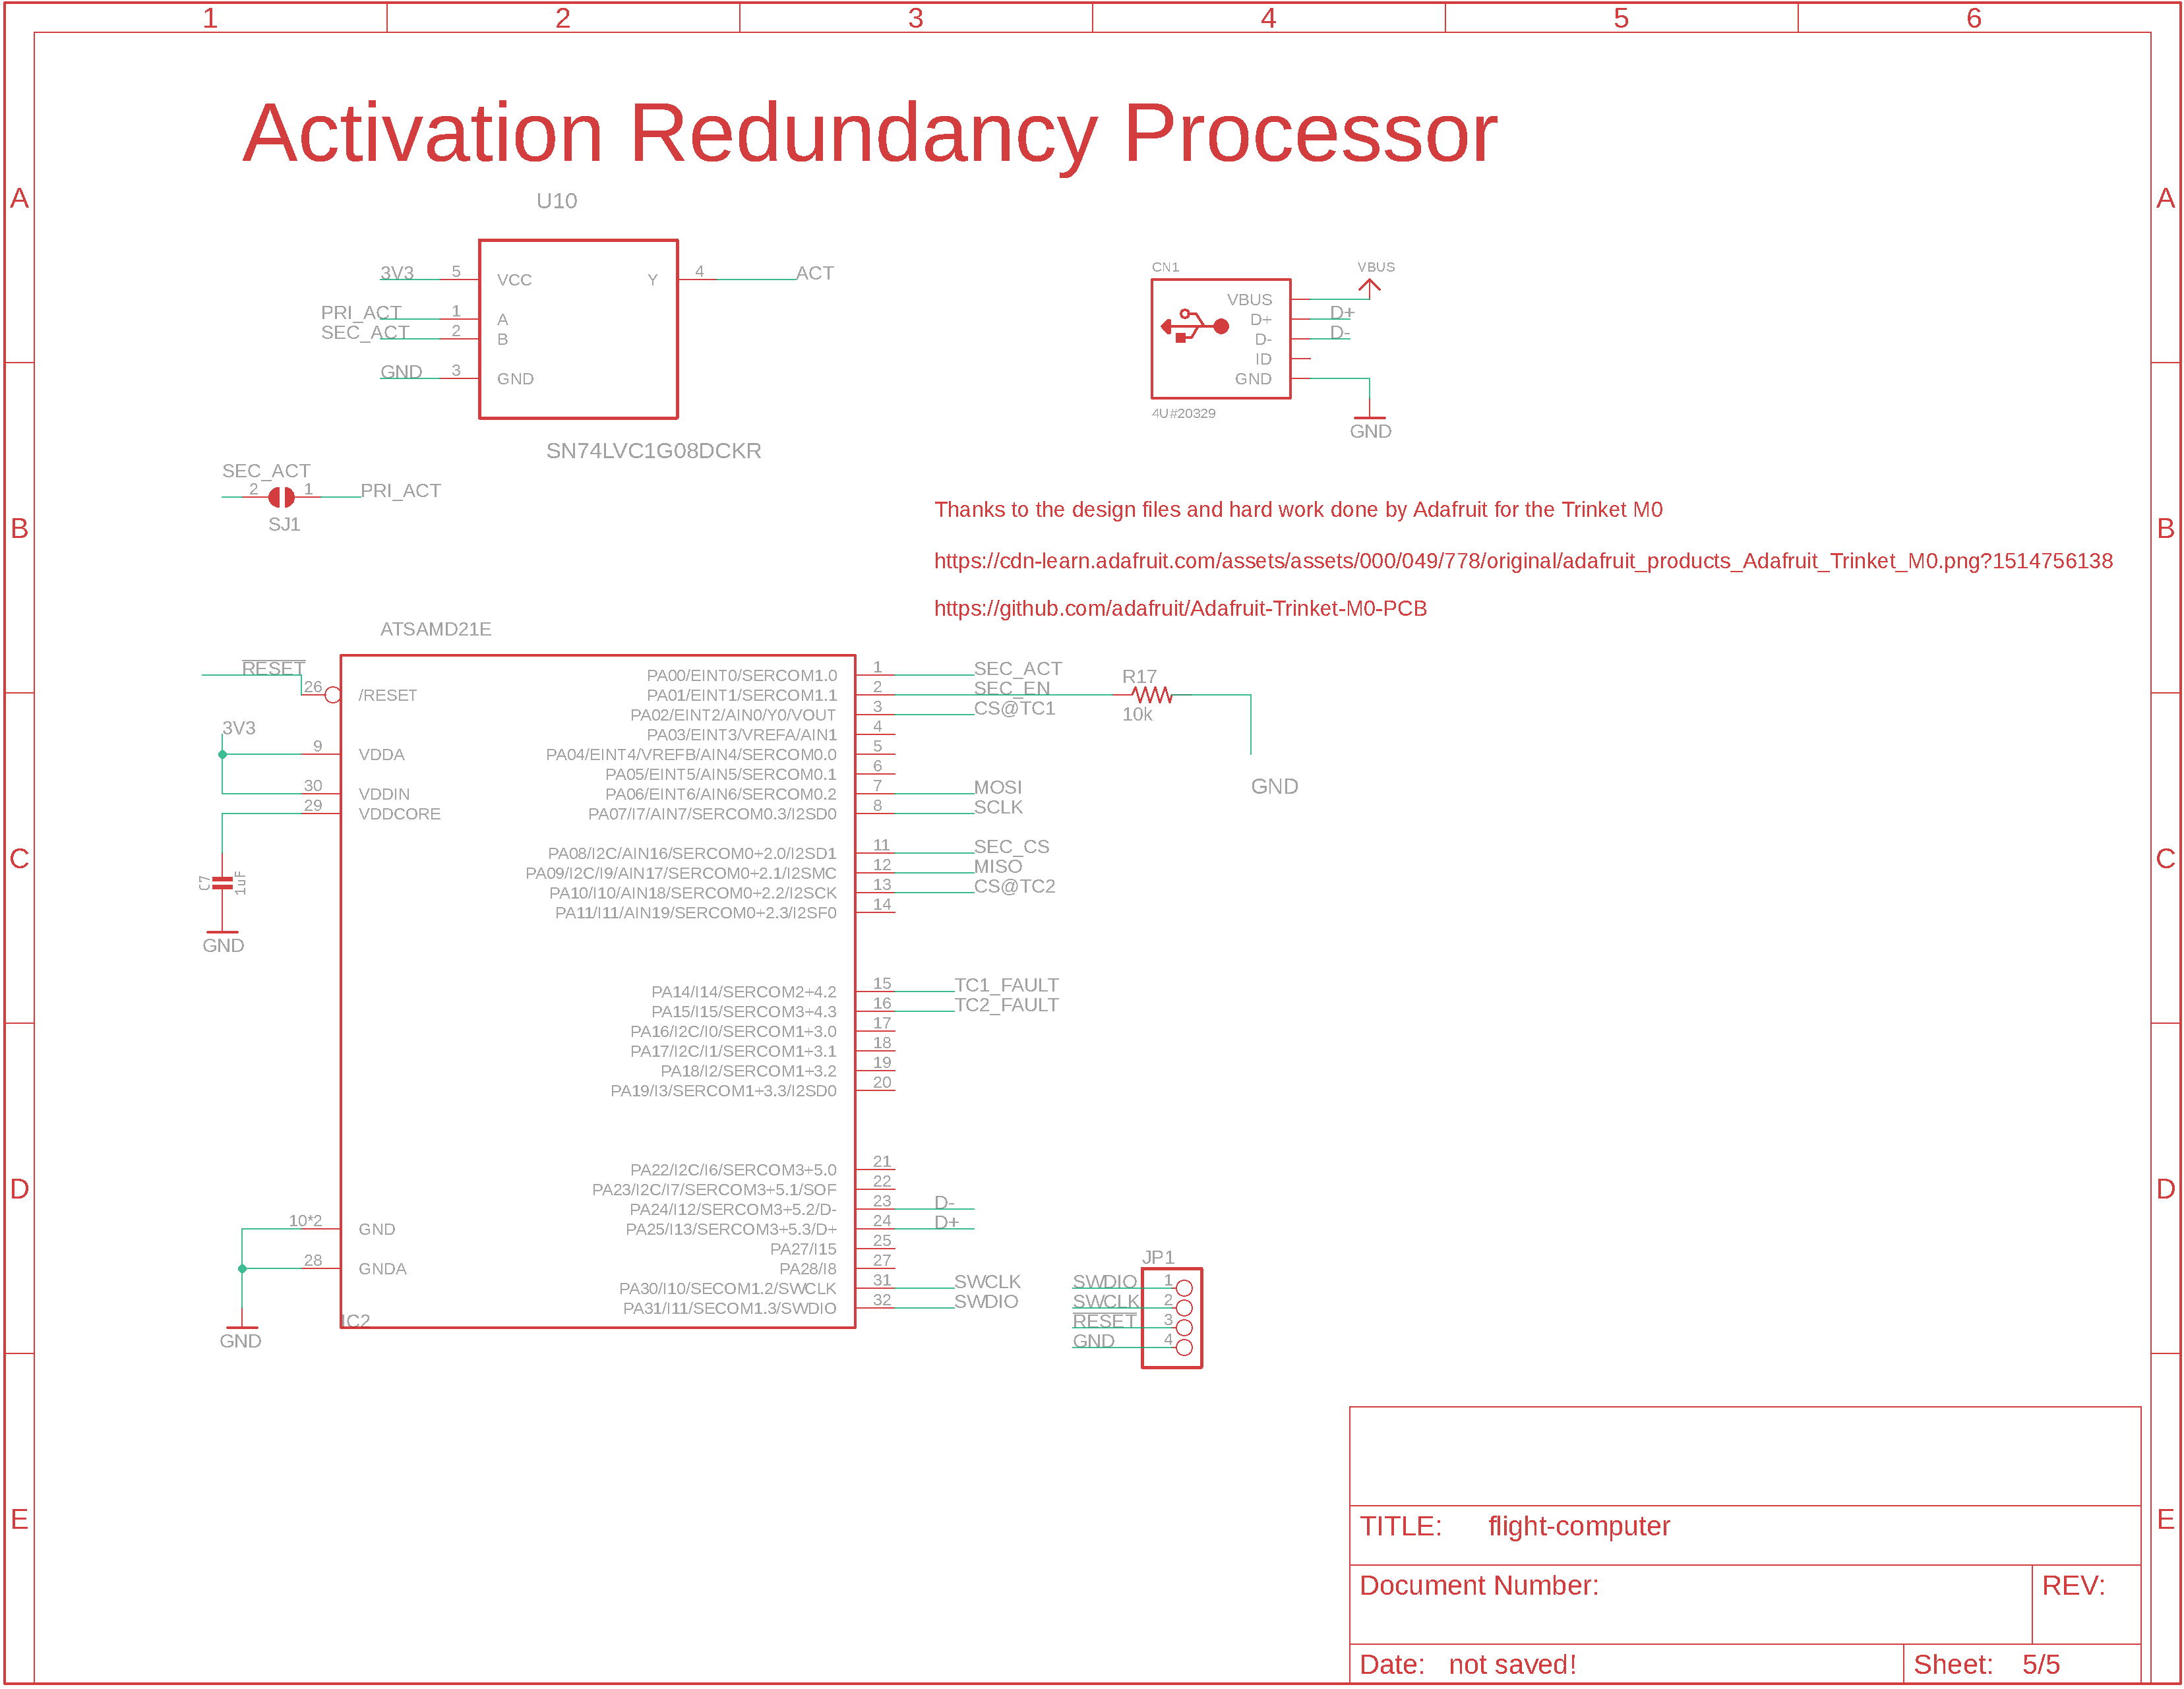
\includegraphics[width=\textwidth]{images/page5.png}
%    \caption{Page five of schematics.}
%    \label{fig:page1-5}
%\end{figure}

\section{Board Renderings}
\begin{figure}[H]
	\centering
	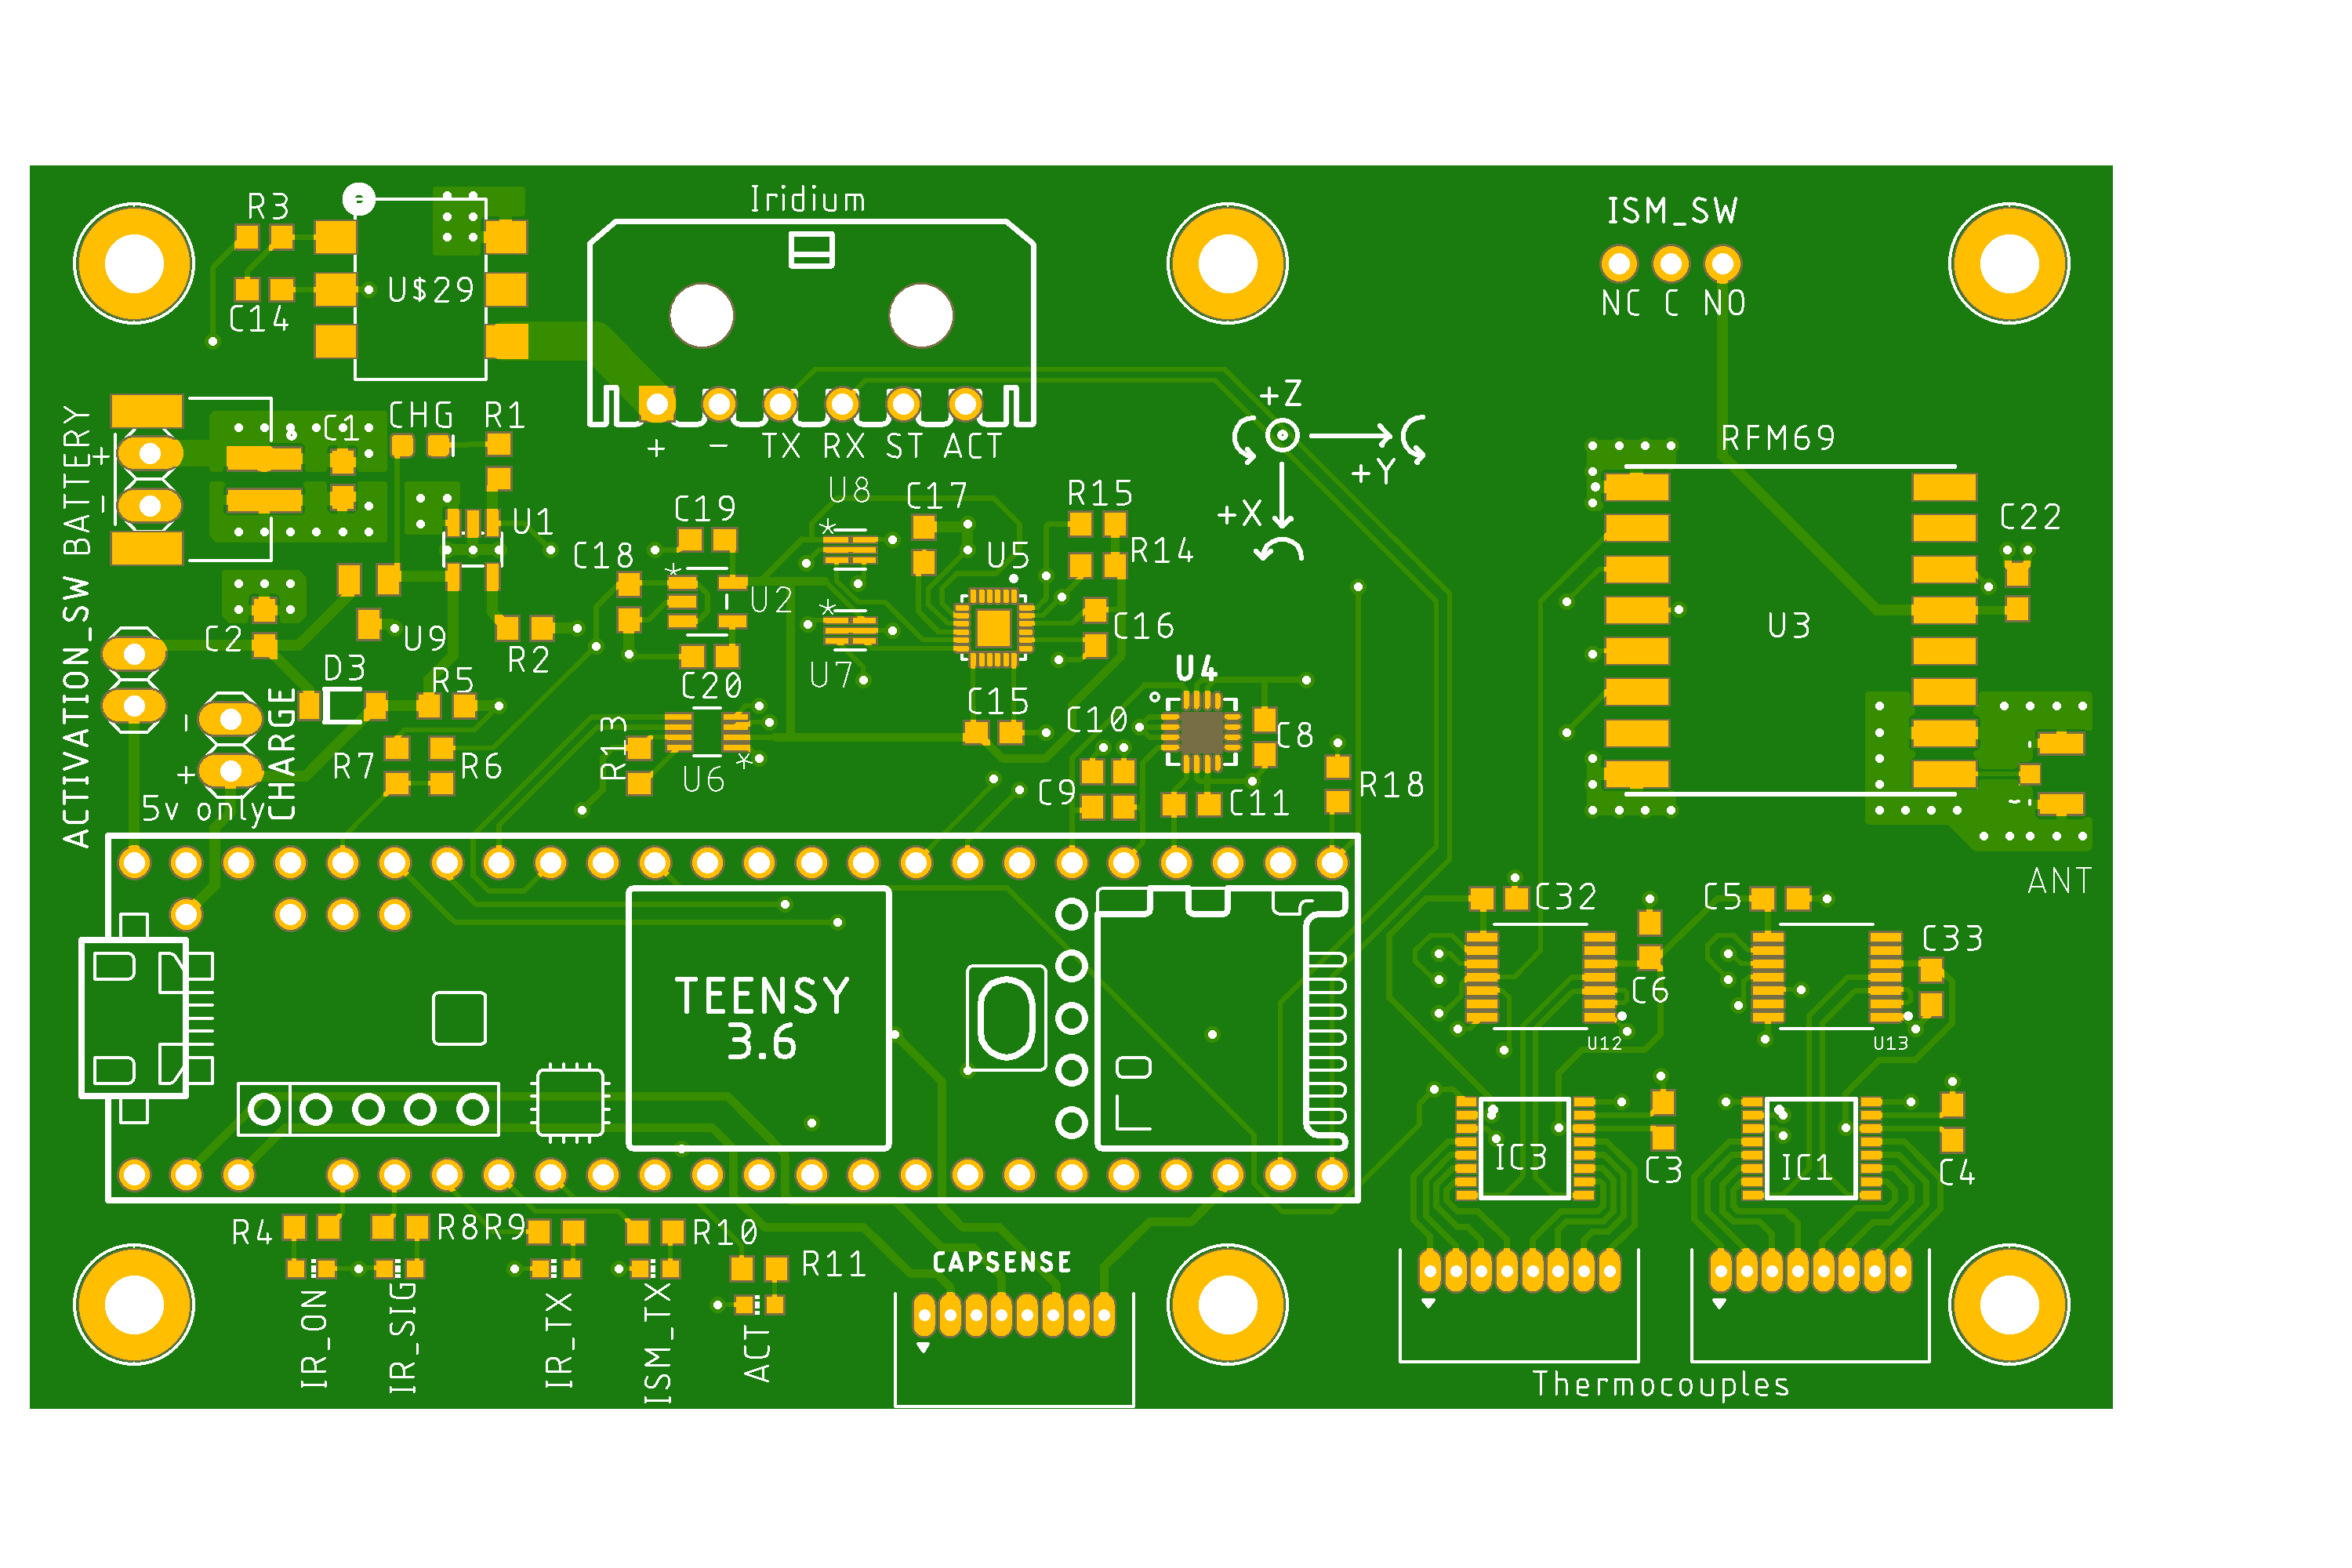
\includegraphics[width=0.9\textwidth]{images/krepe-top.png}
	\caption{Rendering of the top of the KREPE control board, V1.1.}
	\label{fig:board-top}
\end{figure}
\begin{figure}[H]
	\centering
	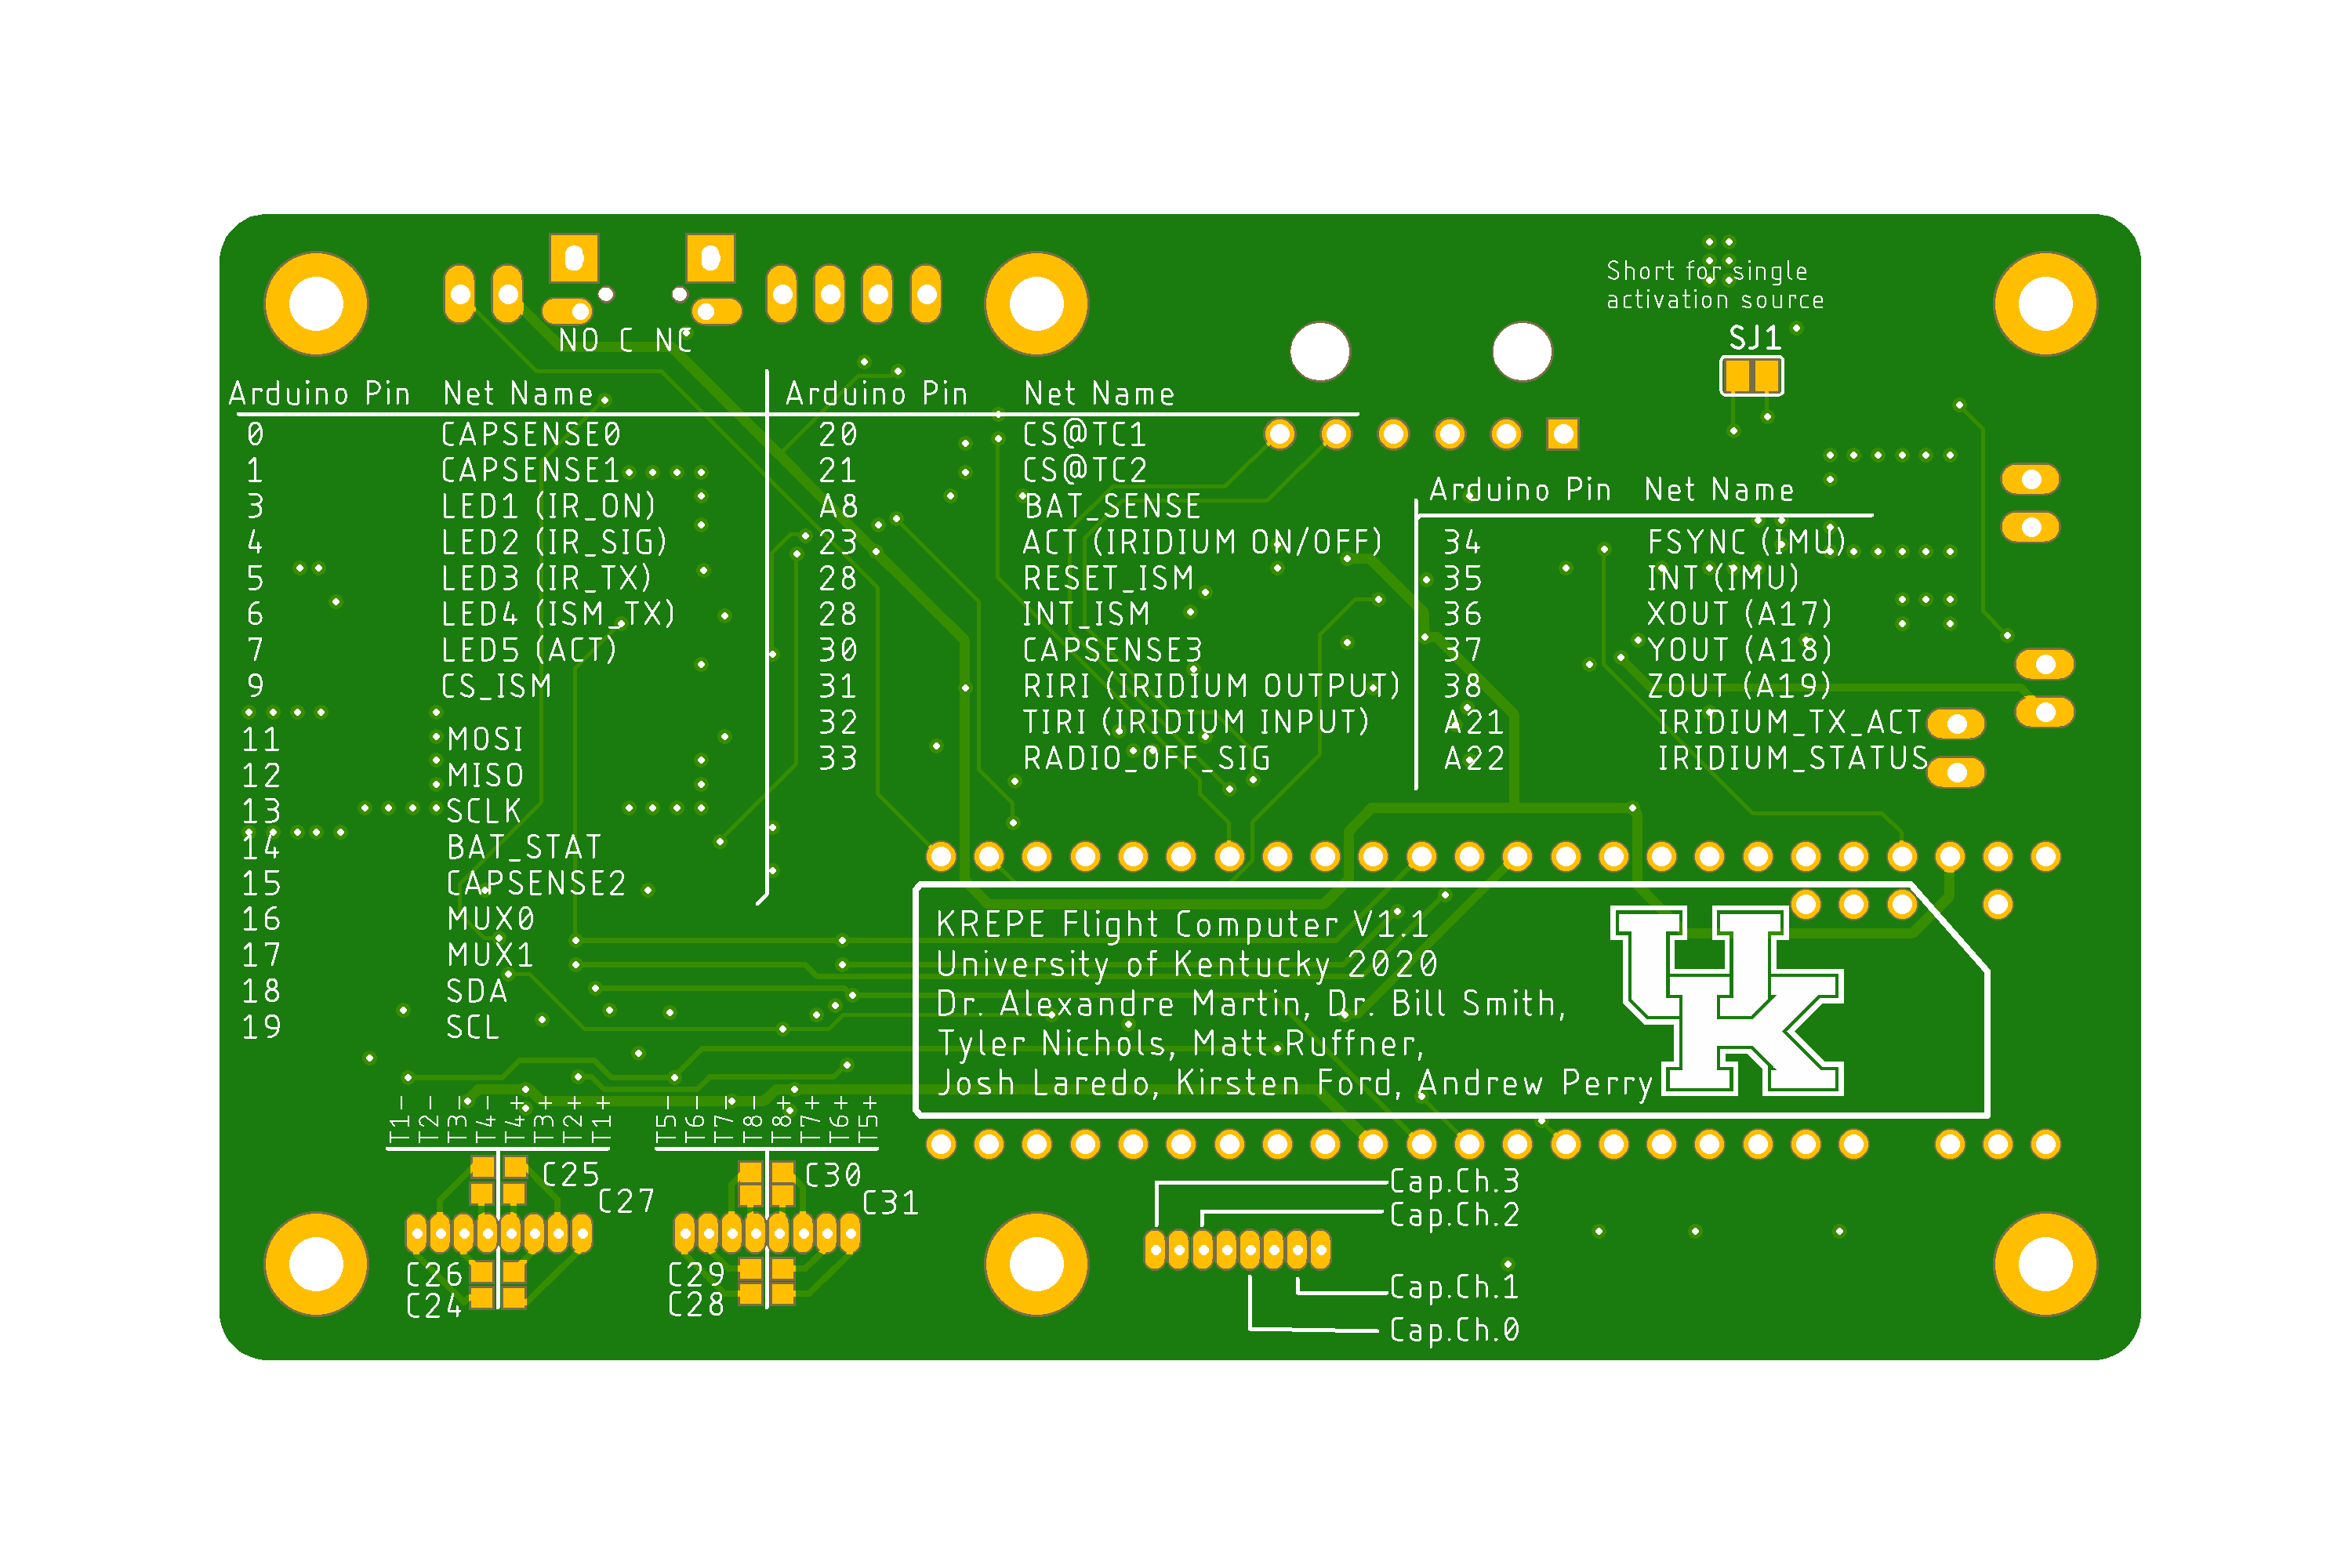
\includegraphics[width=0.9\textwidth]{images/krepe-bottom.png}
	\caption{Rendering of the bottom of the KREPE control board, V1.1.}
	\label{fig:board-bottom}
\end{figure}
%
\section{Teensy 3.5 Reference}
%
\begin{figure}[H]
    \centering
    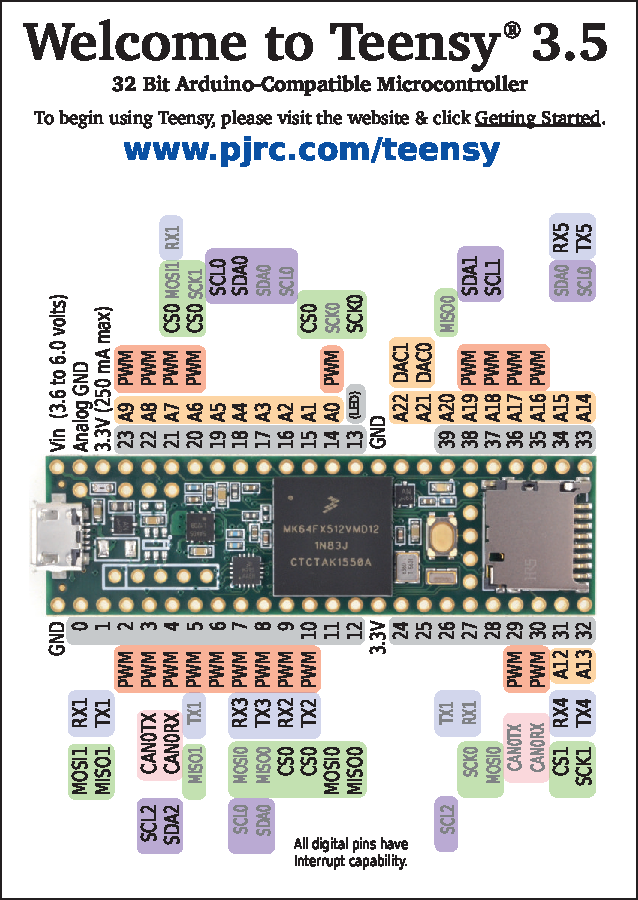
\includegraphics[width=0.8\textwidth]{images/card8a_rev2.pdf}
    \caption{Teensy 3.5 Front}
    \label{fig:teensy-front}
\end{figure}

\begin{figure}[H]
    \centering
    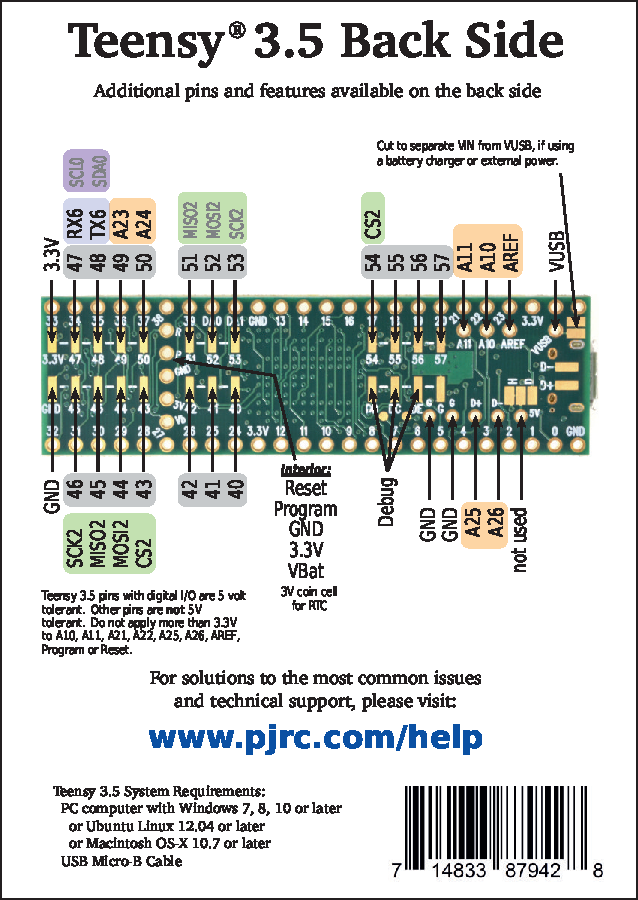
\includegraphics[width=0.8\textwidth]{images/card8b_rev2.pdf}
    \caption{Teensy 3.5 Back}
    \label{fig:teensy-back}
\end{figure}


\begin{figure}[H]
    \centering
    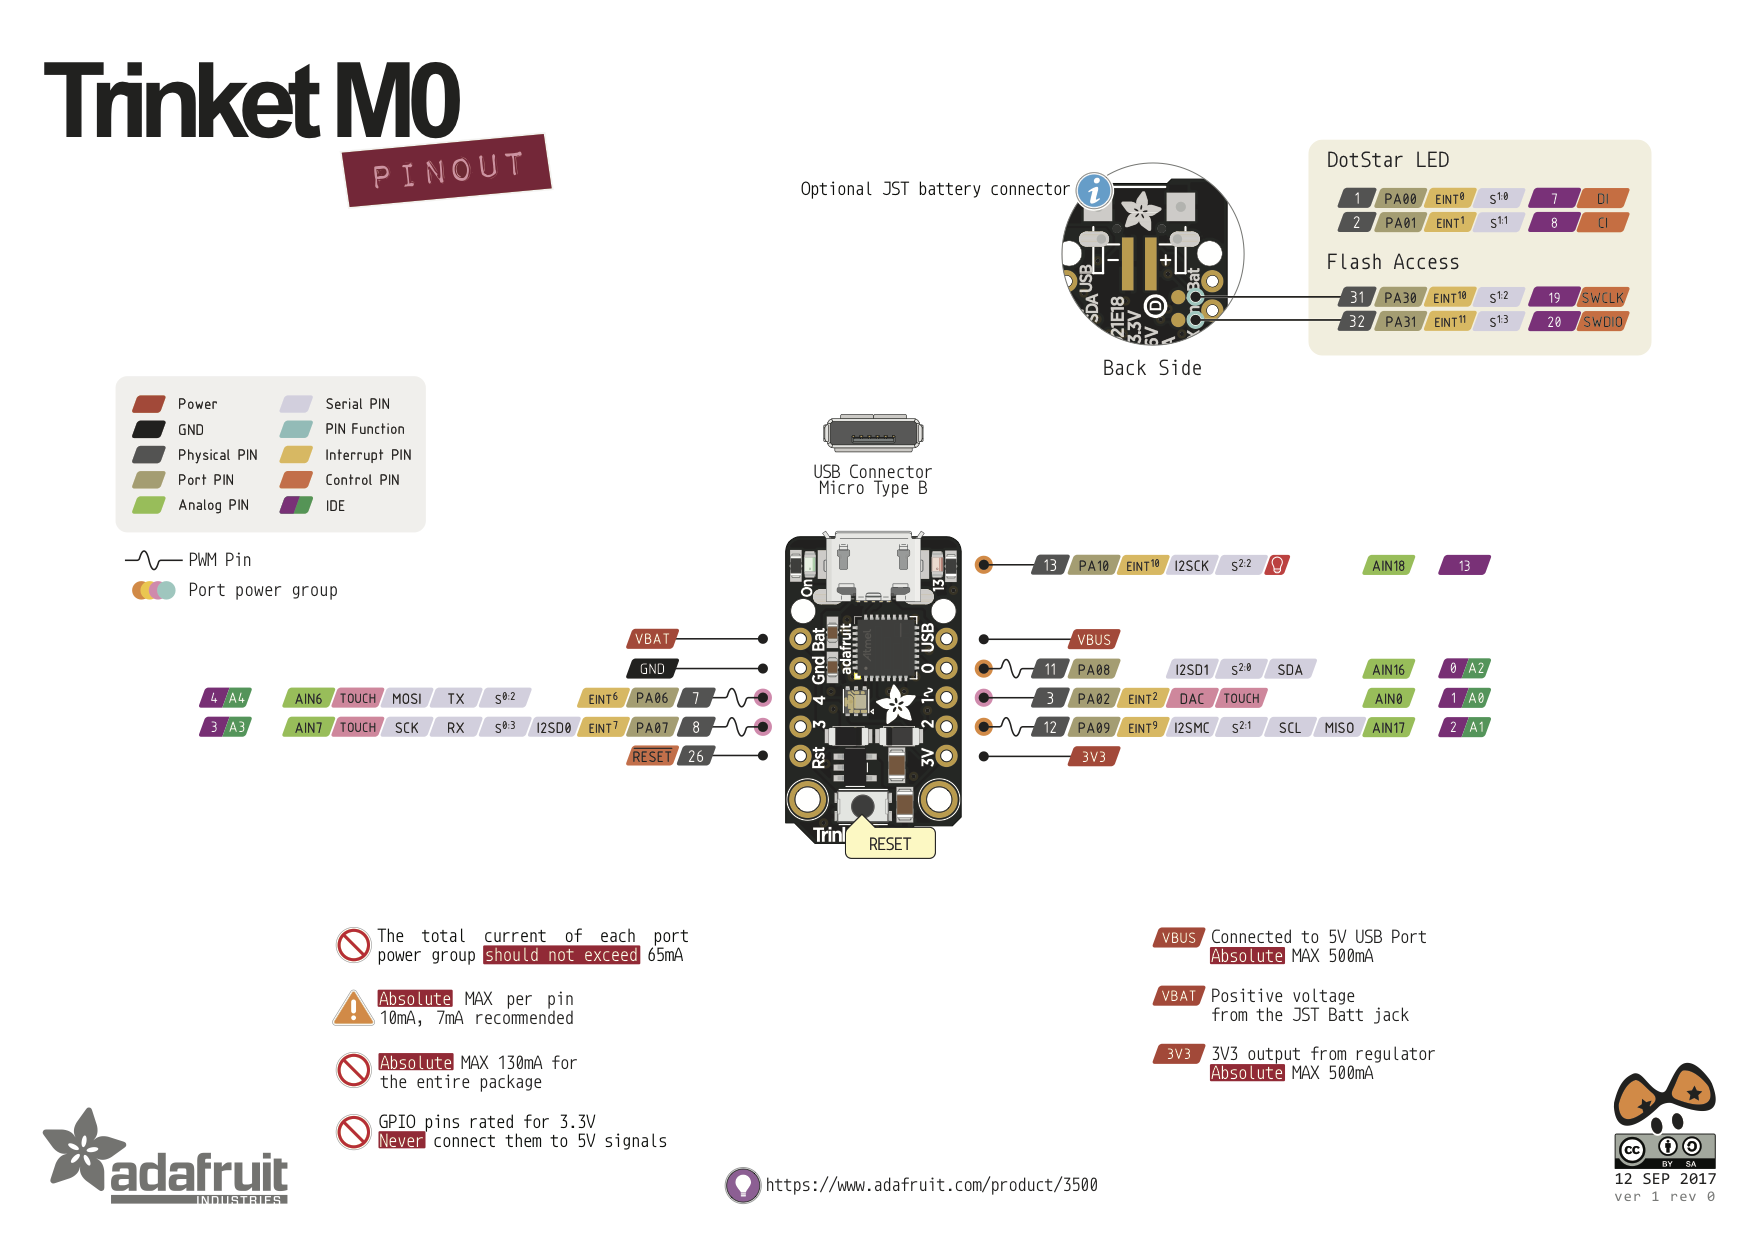
\includegraphics[width=\textwidth]{images/trinket-m0.png}
    \caption{Trinket-M0 Arduino Reference (for ARP chip).}
    \label{fig:trinket-m0}
\end{figure}


\section{Partslist}
\label{app:partslist}
\lstinputlisting[language={},basicstyle=\tiny]{flight-computer-partslist.txt}

\newpage
\section{Arduino Pin Mapping}
\label{app:pinmap}
\lstinputlisting[language={}]{arduino-pinmap.txt}


%% CBCS compliance
\iffalse
\newpage
\section{General Requirements Compliance}
Upon both power up (after primary activation via pull-tab) and detection of a termination or off-nominal power condition, the Teensy processor will enter a safe reset state, where all GPIO pins controlling critical system functions are set to a high impedance value. This high impedance state, in addition to the flight computer PCB, ensure requirements in the \textit{General Requirements for the Computer-Based Control System Safety Requirements for the ISS} are met. Overcurrent and undervoltage protection for battery cells is implemented upstream of the flight computer, limiting the off-nominal power conditions expected (see KREPE Flight Computer Hardware Manual). See Fig. \ref{fig:exec-lifecycle} for an overview of the main execution lifecycle and how upon both power up and detection of an abnormal power condition both put the CBCS back into the safe high impedance state. CBCS General Requirements are discussed below.

\subsection{Req. 3.1.1.1}
Teensy 3.5 controller documentation shows that the controller powers up into the known safe reset state. No outputs occur until the processing state is initiated (see Fig. \ref{fig:exec-lifecycle}). Verification for this requirement will monitor the state of Teensy output pins with external hardware upon power up to make sure specific signals (i.e. iridium soli state relay activation signal) do not transition unexpectedly. 

\subsection{Req. 3.1.1.2}
KREPE flight computer software on the Teensy 3.5 controller enters a safe state in the event that a termination condition is detected (e.g. low system battery  voltage; see Fig. \ref{fig:exec-lifecycle}). As the KREPE capsule is incapable of receiving any external commands, the detection of a termination command scenario is not applicable. Testing for compliance with this requirement entails monitoring of Flight computer pin state with external hardware while the system experiences low battery voltage to make sure it places critical pins in a high impedance or off state.

\subsection{Req. 3.1.1.3}
The KREPE battery protection subsystem prevents any overcurrent or undervoltage conditions from reaching the flight computer. The main off-nominal power condition the flight computer may encounter is power failure. The Teensy 3.5 controller features a power management controller that will place it in a safe reset state if a power failure is detected. The KREPE flight computer also  monitors system battery voltage to preemtively detect an off-nominal power condition and place the system in the safe state (see Fig. \ref{fig:exec-lifecycle}).

Testing of all flown cells will be done including full charge/discharging cycling, under-voltage, over-voltage, and over-current testing with the battery protection circuitry in place. Analysis will be performed via debug interface and external hardware to make sure the flight computer returns to the prescribed safe reset state upon recovery from these off-nominal power conditions.

\begin{figure}
  \centering
  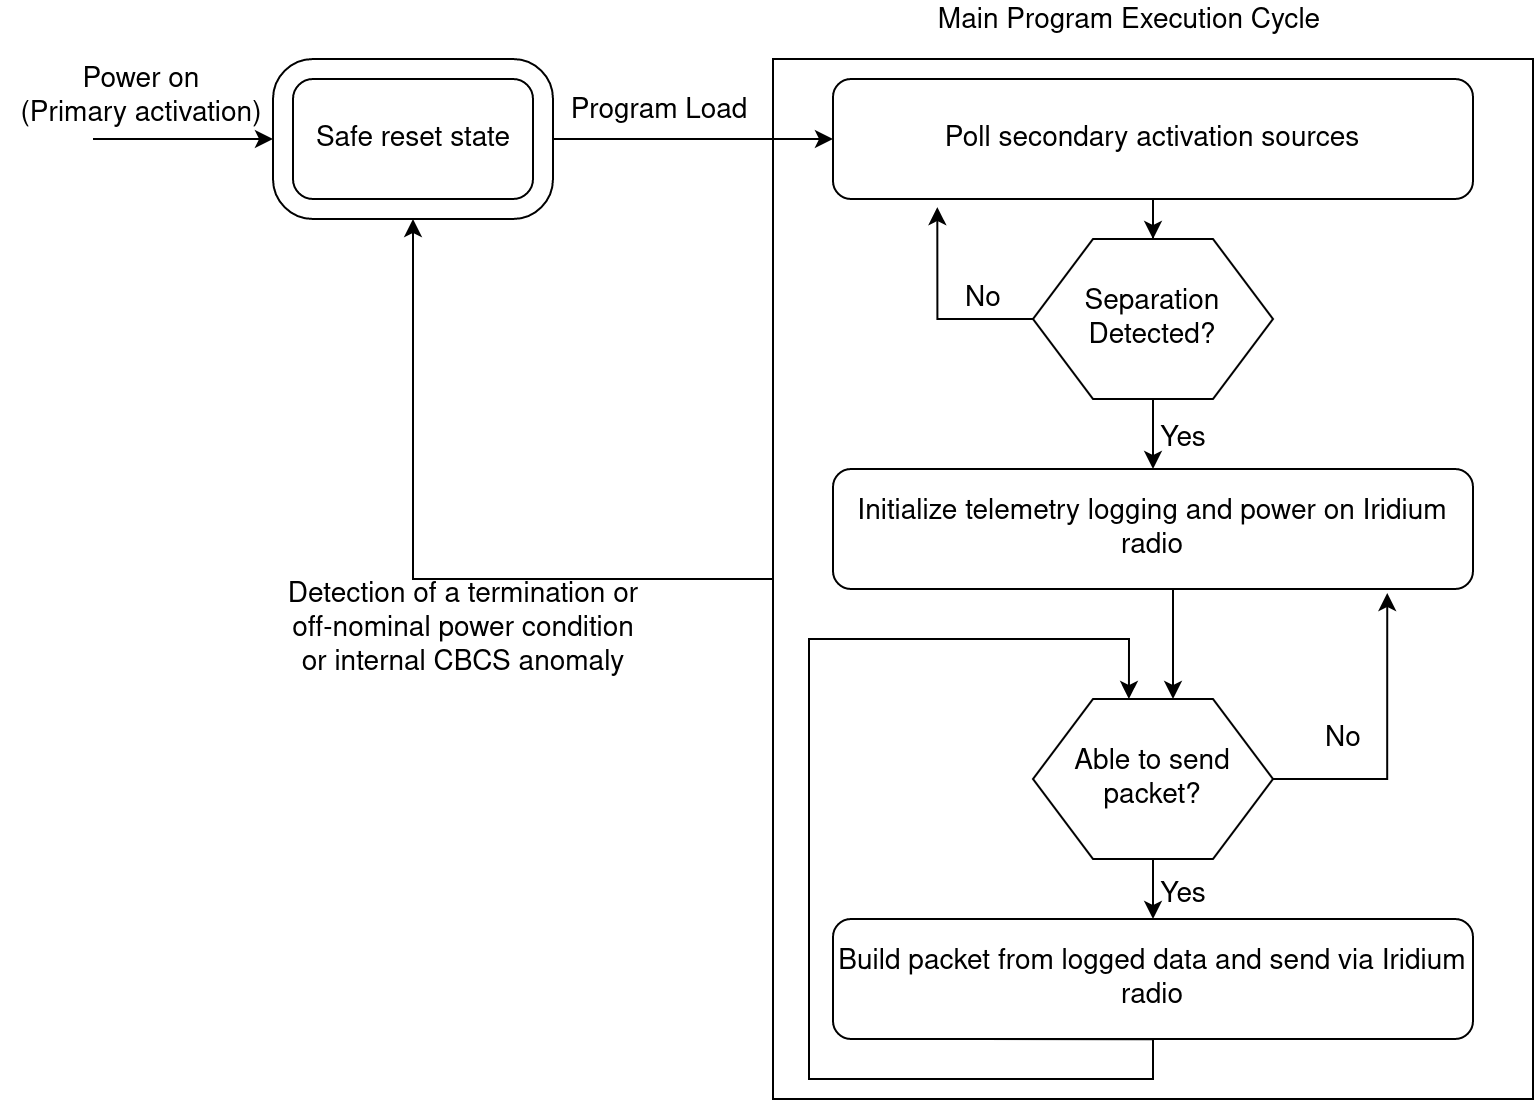
\includegraphics[width=0.75\textwidth]{images/software-overview.png}
  \caption{Overview of main execution cycle showing return to safe high-Z reset state upon startup and abnormal power condition.}
  \label{fig:exec-lifecycle}
\end{figure}

\subsection{3.1.1.4}
N/A

\subsection{3.1.1.5}
N/A

\subsection{3.1.1.6}
The metal enclosure that houses the KREPE module acts as a Faraday cage and mitigates the risk imposed to the CBCS by inadvertent memory modification.
Inspection
See 3.1.1.4
Suggest putting a transmitter inside and see if we can detect any leakage at MSFC if possible.
\subsection{3.1.1.7}
Upon detection of an anomaly internal to the CBCS there is watchdog timer functionality that will return the CBCS to the known safe initialization state. Verification procedures for this requirement entail physical disruption/disconnection of flight computer hardware to ensure control software can recover.

\subsection{3.1.1.8}
The external sources in this case would be the ambient temperature of capsule and the presence of the metal enclosure around the KREPE capsule. The capsule uses the Fault flags on the thermocouple to digital converter are used to discern if a valid thermocouple reading has been collected or not. There are also multiple thermocouples whos values are cross checked for consistency in valid readings.
% Capacitive sensing is also used to detect the presence of the metal enclosure around the KREPE capsule. Both of these inputs are used to discern between valid and invalid input.

%Verification for this requirement entails physical disconnection/perturbation of thermocouple and capacitive sensing leads to analyze the induced effect on measurement values and fault conditions. 

\subsection{3.1.1.9}
Inspection
Inspection of software code verifies all lines of code are traceable to system or software requirements.
Test
Coverage analysis of flight code will ensure lack of dead code and all system software acts for a requirement.
See Fig. \ref{fig:exec-lifecycle} for KREPE software design requirements.

\subsection{3.1.1.10}
All flight software is developed to first meet system requirements. The system requirements outline what functionality will be required from the software as well as what will be available to serve as sources of information. Another consideration that is taken during this phase of software development is the hardware that the software will be running on. As the development cycle gets into writing the software itself, the primary method of configuration management follows a traditional Agile development cycle with team meetings every week to address concerns and defects. The codebase itself is structured and modular in nature so making isolated changes to configure the software to a different hardware or mission spec is controlled and reversible if need be.

Version control is also used to maintain both productivity and preserve proper versioning of the codebase once large sets of requirements are successfully encompassed and have passed testing. For testing and building release versions of the software, all merge requests must be approved by at least 1 other engineer to preserve main version branch functionality and which requirements each version completes will be documented in the repository itself. Verification and validation processes happen under formal testing conditions when hardware is readily available to run simulated mission conditions and ensure the checklist of requirements is fulfilled. 

\subsection{3.1.1.11}
N/A - the single board design of the KREPE module is designed such that complicated transmission and reception lines between devices, e.g. 1553  busses, are not necessary.

\subsection{3.1.1.12}
N/A - KREPE has no requirement for audio communication. KREPE has no uplink capability, therefore unauthorized third party control is not possible for KREPE.

\subsection{3.1.1.13}
N/A - KREPE does not receive any commands.
\fi

%\bibliographystyle{plain}
%\bibliography{references}
\end{document}
